\newcommand{\CLASSINPUTbottomtextmargin}{1in}
\documentclass[letterpaper,onecolumn,draftcls]{IEEEtran}
%\documentclass[conference,a4paper]{IEEEtran}
\usepackage[ruled,vlined,linesnumbered]{algorithm2e}
\usepackage[noend]{algpseudocode}

%\usepackage[OT1,T1]{fontenc}

\usepackage[numbers,sort&compress]{natbib}
\renewcommand{\bibfont}{\footnotesize}
%\usepackage{cite}
%\usepackage{mystyle}
%%%%%%%%%%%%%%%%%%%%%%%%%%%%%%%%%%%%
\makeatletter

\usepackage{etex}

%%% Review %%%

\usepackage{zref-savepos}

\newcounter{mnote}%[page]
\renewcommand{\themnote}{p.\thepage\;$\langle$\arabic{mnote}$\rangle$}

\def\xmarginnote{%
  \xymarginnote{\hskip -\marginparsep \hskip -\marginparwidth}}

\def\ymarginnote{%
  \xymarginnote{\hskip\columnwidth \hskip\marginparsep}}

\long\def\xymarginnote#1#2{%
\vadjust{#1%
\smash{\hbox{{%
        \hsize\marginparwidth
        \@parboxrestore
        \@marginparreset
\footnotesize #2}}}}}

\def\mnoteson{%
\gdef\mnote##1{\refstepcounter{mnote}\label{##1}%
  \zsavepos{##1}%
  \ifnum20432158>\number\zposx{##1}%
  \xmarginnote{{\color{blue}\bf $\langle$\arabic{mnote}$\rangle$}}% 
  \else
  \ymarginnote{{\color{blue}\bf $\langle$\arabic{mnote}$\rangle$}}%
  \fi%
}
  }
\gdef\mnotesoff{\gdef\mnote##1{}}
\mnoteson
\mnotesoff








%%% Layout %%%

% \usepackage{geometry} % override layout
% \geometry{tmargin=2.5cm,bmargin=m2.5cm,lmargin=3cm,rmargin=3cm}
% \setlength{\pdfpagewidth}{8.5in} % overrides default pdftex paper size
% \setlength{\pdfpageheight}{11in}

\newlength{\mywidth}

%%% Conventions %%%

% References
\newcommand{\figref}[1]{Fig.~\ref{#1}}
\newcommand{\defref}[1]{Definition~\ref{#1}}
\newcommand{\tabref}[1]{Table~\ref{#1}}
% general
%\usepackage{ifthen,nonfloat,subfigure,rotating,array,framed}
\usepackage{framed}
%\usepackage{subfigure}
\usepackage{subcaption}
\usepackage{comment}
%\specialcomment{nb}{\begingroup \noindent \framed\textbf{n.b.\ }}{\endframed\endgroup}
%%\usepackage{xtab,arydshln,multirow}
% topcaption defined in xtab. must load nonfloat before xtab
%\PassOptionsToPackage{svgnames,dvipsnames}{xcolor}
\usepackage[svgnames,dvipsnames]{xcolor}
%\definecolor{myblue}{rgb}{.8,.8,1}
%\definecolor{umbra}{rgb}{.8,.8,.5}
%\newcommand*\mybluebox[1]{%
%  \colorbox{myblue}{\hspace{1em}#1\hspace{1em}}}
\usepackage[all]{xy}
%\usepackage{pstricks,pst-node}
\usepackage{tikz}
\usetikzlibrary{positioning,matrix,through,calc,arrows,fit,shapes,decorations.pathreplacing,decorations.markings,}

\tikzstyle{block} = [draw,fill=blue!20,minimum size=2em]



% typsetting math
\usepackage{qsymbols,amssymb,mathrsfs}
\usepackage{amsmath}
\usepackage[standard,thmmarks]{ntheorem}
\theoremstyle{plain}
\theoremsymbol{\ensuremath{_\vartriangleleft}}
\theorembodyfont{\itshape}
\theoremheaderfont{\normalfont\bfseries}
\theoremseparator{}
\newtheorem{Claim}{Claim}
\newtheorem{Subclaim}{Subclaim}
\theoremstyle{nonumberplain}
\theoremheaderfont{\scshape}
\theorembodyfont{\normalfont}
\theoremsymbol{\ensuremath{_\blacktriangleleft}}
\newtheorem{Subproof}{Proof}

\theoremnumbering{arabic}
\theoremstyle{plain}
\usepackage{latexsym}
\theoremsymbol{\ensuremath{_\Box}}
\theorembodyfont{\itshape}
\theoremheaderfont{\normalfont\bfseries}
\theoremseparator{}
\newtheorem{Conjecture}{Conjecture}

\theorembodyfont{\upshape}
\theoremprework{\bigskip\hrule}
\theorempostwork{\hrule\bigskip}
\newtheorem{Condition}{Condition}%[section]


%\RequirePckage{amsmath} loaded by empheq
\usepackage[overload]{empheq} % no \intertext and \displaybreak
%\usepackage{breqn}

\let\iftwocolumn\if@twocolumn
\g@addto@macro\@twocolumntrue{\let\iftwocolumn\if@twocolumn}
\g@addto@macro\@twocolumnfalse{\let\iftwocolumn\if@twocolumn}

%\empheqset{box=\mybluebox}
%\usepackage{mathtools}      % to polish math typsetting, loaded
%                                % by empeq
\mathtoolsset{showonlyrefs=false,showmanualtags}
\let\underbrace\LaTeXunderbrace % adapt spacing to font sizes
\let\overbrace\LaTeXoverbrace
\renewcommand{\eqref}[1]{\textup{(\refeq{#1})}} % eqref was not allowed in
                                       % sub/super-scripts
\newtagform{brackets}[]{(}{)}   % new tags for equations
\usetagform{brackets}
% defined commands:
% \shortintertext{}, dcases*, \cramped, \smashoperator[]{}

\usepackage[Smaller]{cancel}
\renewcommand{\CancelColor}{\color{Red}}
%\newcommand\hcancel[2][black]{\setbox0=\hbox{#2}% colored horizontal cross
%  \rlap{\raisebox{.45\ht0}{\color{#1}\rule{\wd0}{1pt}}}#2}

% hyperlink
\PassOptionsToPackage{breaklinks,hyperindex=true,backref=false,bookmarksnumbered,bookmarksopen,linktocpage,colorlinks,linkcolor=BrickRed,citecolor=OliveGreen,urlcolor=Blue,pdfstartview=FitH}{hyperref}
\usepackage{hyperref}


% makeindex style
\newcommand{\indexmain}[1]{\textbf{\hyperpage{#1}}}

\usepackage{graphicx,psfrag}
\graphicspath{{figure/}{image/}} % Search path of figures

% for tabular
\usepackage{diagbox} % \backslashbox{}{} for slashed entries
%\usepackage{threeparttable} % threeparttable, \tnote{},
                                % tablenotes, and \item[]
%\usepackage{colortab} % \cellcolor[gray]{0.9},
%\rowcolor,\columncolor,
%\usepackage{colortab} % \LCC \gray & ...  \ECC \\

% typesetting codes
%\usepackage{maple2e} % need to use \char29 for ^
\usepackage{algorithm2e}
\usepackage{listings} 
\lstdefinelanguage{Maple}{
  morekeywords={proc,module,end, for,from,to,by,while,in,do,od
    ,if,elif,else,then,fi ,use,try,catch,finally}, sensitive,
  morecomment=[l]\#,
  morestring=[b]",morestring=[b]`}[keywords,comments,strings]
\lstset{
  basicstyle=\scriptsize,
  keywordstyle=\color{ForestGreen}\bfseries,
  commentstyle=\color{DarkBlue},
  stringstyle=\color{DimGray}\ttfamily,
  texcl
}
%%% New fonts %%%
\DeclareMathAlphabet{\mathpzc}{OT1}{pzc}{m}{it}
\usepackage{upgreek} % \upalpha,\upbeta, ...
%\usepackage{bbold}   % blackboard math
\usepackage{dsfont}  % \mathds

%%% Macros for multiple definitions %%%

% example usage:
% \multi{M}{\boldsymbol{#1}}  % defines \multiM
% \multi ABC.                 % defines \MA \MB and \MC as
%                             % \boldsymbol{A}, \boldsymbol{B} and
%                             % \boldsymbol{C} respectively.
% 
%  The last period '.' is necessary to terminate the macro expansion.
%
% \multi*{M}{\boldsymbol{#1}} % defines \multiM and \M
% \M{A}                       % expands to \boldsymbol{A}

\def\multi@nostar#1#2{%
  \expandafter\def\csname multi#1\endcsname##1{%
    \if ##1.\let\next=\relax \else
    \def\next{\csname multi#1\endcsname}     
    %\expandafter\def\csname #1##1\endcsname{#2}
    \expandafter\newcommand\csname #1##1\endcsname{#2}
    \fi\next}}

\def\multi@star#1#2{%
  \expandafter\def\csname #1\endcsname##1{#2}
  \multi@nostar{#1}{#2}
}

\newcommand{\multi}{%
  \@ifstar \multi@star \multi@nostar}

%%% new alphabets %%%

\multi*{rm}{\mathrm{#1}}
\multi*{mc}{\mathcal{#1}}
\multi*{op}{\mathop {\operator@font #1}}
% \multi*{op}{\operatorname{#1}}
\multi*{ds}{\mathds{#1}}
\multi*{set}{\mathcal{#1}}
\multi*{rsfs}{\mathscr{#1}}
\multi*{pz}{\mathpzc{#1}}
\multi*{M}{\boldsymbol{#1}}
\multi*{R}{\mathsf{#1}}
\multi*{RM}{\M{\R{#1}}}
\multi*{bb}{\mathbb{#1}}
\multi*{td}{\tilde{#1}}
\multi*{tR}{\tilde{\mathsf{#1}}}
\multi*{trM}{\tilde{\M{\R{#1}}}}
\multi*{tset}{\tilde{\mathcal{#1}}}
\multi*{tM}{\tilde{\M{#1}}}
\multi*{baM}{\bar{\M{#1}}}
\multi*{ol}{\overline{#1}}

\multirm  ABCDEFGHIJKLMNOPQRSTUVWXYZabcdefghijklmnopqrstuvwxyz.
\multiol  ABCDEFGHIJKLMNOPQRSTUVWXYZabcdefghijklmnopqrstuvwxyz.
\multitR   ABCDEFGHIJKLMNOPQRSTUVWXYZabcdefghijklmnopqrstuvwxyz.
\multitd   ABCDEFGHIJKLMNOPQRSTUVWXYZabcdefghijklmnopqrstuvwxyz.
\multitset ABCDEFGHIJKLMNOPQRSTUVWXYZabcdefghijklmnopqrstuvwxyz.
\multitM   ABCDEFGHIJKLMNOPQRSTUVWXYZabcdefghijklmnopqrstuvwxyz.
\multibaM   ABCDEFGHIJKLMNOPQRSTUVWXYZabcdefghijklmnopqrstuvwxyz.
\multitrM   ABCDEFGHIJKLMNOPQRSTUVWXYZabcdefghijklmnopqrstuvwxyz.
\multimc   ABCDEFGHIJKLMNOPQRSTUVWXYZabcdefghijklmnopqrstuvwxyz.
\multiop   ABCDEFGHIJKLMNOPQRSTUVWXYZabcdefghijklmnopqrstuvwxyz.
\multids   ABCDEFGHIJKLMNOPQRSTUVWXYZabcdefghijklmnopqrstuvwxyz.
\multiset  ABCDEFGHIJKLMNOPQRSTUVWXYZabcdefghijklmnopqrstuvwxyz.
\multirsfs ABCDEFGHIJKLMNOPQRSTUVWXYZabcdefghijklmnopqrstuvwxyz.
\multipz   ABCDEFGHIJKLMNOPQRSTUVWXYZabcdefghijklmnopqrstuvwxyz.
\multiM    ABCDEFGHIJKLMNOPQRSTUVWXYZabcdefghijklmnopqrstuvwxyz.
\multiR    ABCDEFGHIJKL NO QR TUVWXYZabcd fghijklmnopqrstuvwxyz.
\multibb   ABCDEFGHIJKLMNOPQRSTUVWXYZabcdefghijklmnopqrstuvwxyz.
\multiRM   ABCDEFGHIJKLMNOPQRSTUVWXYZabcdefghijklmnopqrstuvwxyz.
\newcommand{\RRM}{\R{M}}
\newcommand{\RRP}{\R{P}}
\newcommand{\RRe}{\R{e}}
\newcommand{\RRS}{\R{S}}
%%% new symbols %%%

%\newcommand{\dotgeq}{\buildrel \textstyle  .\over \geq}
%\newcommand{\dotleq}{\buildrel \textstyle  .\over \leq}
\newcommand{\dotleq}{\buildrel \textstyle  .\over {\smash{\lower
      .2ex\hbox{\ensuremath\leqslant}}\vphantom{=}}}
\newcommand{\dotgeq}{\buildrel \textstyle  .\over {\smash{\lower
      .2ex\hbox{\ensuremath\geqslant}}\vphantom{=}}}

\DeclareMathOperator*{\argmin}{arg\,min}
\DeclareMathOperator*{\argmax}{arg\,max}

%%% abbreviations %%%

% commands
\newcommand{\esm}{\ensuremath}

% environments
\newcommand{\bM}{\begin{bmatrix}}
\newcommand{\eM}{\end{bmatrix}}
\newcommand{\bSM}{\left[\begin{smallmatrix}}
\newcommand{\eSM}{\end{smallmatrix}\right]}
\renewcommand*\env@matrix[1][*\c@MaxMatrixCols c]{%
  \hskip -\arraycolsep
  \let\@ifnextchar\new@ifnextchar
  \array{#1}}



% sets of number
\newqsymbol{`N}{\mathbb{N}}
\newqsymbol{`R}{\mathbb{R}}
\newqsymbol{`P}{\mathbb{P}}
\newqsymbol{`Z}{\mathbb{Z}}

% symbol short cut
\newqsymbol{`|}{\mid}
% use \| for \parallel
\newqsymbol{`8}{\infty}
\newqsymbol{`1}{\left}
\newqsymbol{`2}{\right}
\newqsymbol{`6}{\partial}
\newqsymbol{`0}{\emptyset}
\newqsymbol{`-}{\leftrightarrow}
\newqsymbol{`<}{\langle}
\newqsymbol{`>}{\rangle}

%%% new operators / functions %%%

\newcommand{\sgn}{\operatorname{sgn}}
\newcommand{\Var}{\op{Var}}
\newcommand{\diag}{\operatorname{diag}}
\newcommand{\erf}{\operatorname{erf}}
\newcommand{\erfc}{\operatorname{erfc}}
\newcommand{\erfi}{\operatorname{erfi}}
\newcommand{\adj}{\operatorname{adj}}
\newcommand{\supp}{\operatorname{supp}}
\newcommand{\E}{\opE\nolimits}
\newcommand{\T}{\intercal}
% requires mathtools
% \abs,\abs*,\abs[<size_cmd:\big,\Big,\bigg,\Bigg etc.>]
\DeclarePairedDelimiter\abs{\lvert}{\rvert} 
\DeclarePairedDelimiter\norm{\lVert}{\rVert}
\DeclarePairedDelimiter\ceil{\lceil}{\rceil}
\DeclarePairedDelimiter\floor{\lfloor}{\rfloor}
\DeclarePairedDelimiter\Set{\{}{\}}
\newcommand{\imod}[1]{\allowbreak\mkern10mu({\operator@font mod}\,\,#1)}

%%% new formats %%%
\newcommand{\leftexp}[2]{{\vphantom{#2}}^{#1}{#2}}


% non-floating figures that can be put inside tables
\newenvironment{nffigure}[1][\relax]{\vskip \intextsep
  \noindent\minipage{\linewidth}\def\@captype{figure}}{\endminipage\vskip \intextsep}

\newcommand{\threecols}[3]{
\hbox to \textwidth{%
      \normalfont\rlap{\parbox[b]{\textwidth}{\raggedright#1\strut}}%
        \hss\parbox[b]{\textwidth}{\centering#2\strut}\hss
        \llap{\parbox[b]{\textwidth}{\raggedleft#3\strut}}%
    }% hbox 
}

\newcommand{\reason}[2][\relax]{
  \ifthenelse{\equal{#1}{\relax}}{
    \left(\text{#2}\right)
  }{
    \left(\parbox{#1}{\raggedright #2}\right)
  }
}

\newcommand{\marginlabel}[1]
{\mbox[]\marginpar{\color{ForestGreen} \sffamily \small \raggedright\hspace{0pt}#1}}


% up-tag an equation
\newcommand{\utag}[2]{\mathop{#2}\limits^{\text{(#1)}}}
\newcommand{\uref}[1]{(#1)}


% Notation table

\newcommand{\Hline}{\noalign{\vskip 0.1in \hrule height 0.1pt \vskip
    0.1in}}
  
\def\Malign#1{\tabskip=0in
  \halign to\columnwidth{
    \ensuremath{\displaystyle ##}\hfil
    \tabskip=0in plus 1 fil minus 1 fil
    &
    \parbox[t]{0.8\columnwidth}{##}
    \tabskip=0in
    \cr #1}}


%%%%%%%%%%%%%%%%%%%%%%%%%%%%%%%%%%%%%%%%%%%%%%%%%%%%%%%%%%%%%%%%%%%
% MISCELLANEOUS

% Modification from braket.sty by Donald Arseneau
% Command defined is: \extendvert{ }
% The "small versions" use fixed-size brackets independent of their
% contents, whereas the expand the first vertical line '|' or '\|' to
% envelop the content
\let\SavedDoubleVert\relax
\let\protect\relax
{\catcode`\|=\active
  \xdef\extendvert{\protect\expandafter\noexpand\csname extendvert \endcsname}
  \expandafter\gdef\csname extendvert \endcsname#1{\mskip-5mu \left.%
      \ifx\SavedDoubleVert\relax \let\SavedDoubleVert\|\fi
     \:{\let\|\SetDoubleVert
       \mathcode`\|32768\let|\SetVert
     #1}\:\right.\mskip-5mu}
}
\def\SetVert{\@ifnextchar|{\|\@gobble}% turn || into \|
    {\egroup\;\mid@vertical\;\bgroup}}
\def\SetDoubleVert{\egroup\;\mid@dblvertical\;\bgroup}

% If the user is using e-TeX with its \middle primitive, use that for
% verticals instead of \vrule.
%
\begingroup
 \edef\@tempa{\meaning\middle}
 \edef\@tempb{\string\middle}
\expandafter \endgroup \ifx\@tempa\@tempb
 \def\mid@vertical{\middle|}
 \def\mid@dblvertical{\middle\SavedDoubleVert}
\else
 \def\mid@vertical{\mskip1mu\vrule\mskip1mu}
 \def\mid@dblvertical{\mskip1mu\vrule\mskip2.5mu\vrule\mskip1mu}
\fi

%%%%%%%%%%%%%%%%%%%%%%%%%%%%%%%%%%%%%%%%%%%%%%%%%%%%%%%%%%%%%%%%

\makeatother

%%%%%%%%%%%%%%%%%%%%%%%%%%%%%%%%%%%%

\usepackage{ctable}
\usepackage{fouridx}
%\usepackage{calc}
\usepackage{framed}
\usetikzlibrary{positioning,matrix}

\usepackage{paralist}
%\usepackage{refcheck}
\usepackage{enumerate}

\usepackage[normalem]{ulem}
\newcommand{\Ans}[1]{\uuline{\raisebox{.15em}{#1}}}



\numberwithin{equation}{section}
\makeatletter
\@addtoreset{equation}{section}
\renewcommand{\theequation}{\arabic{section}.\arabic{equation}}
\@addtoreset{Theorem}{section}
\renewcommand{\theTheorem}{\arabic{section}.\arabic{Theorem}}
\@addtoreset{Lemma}{section}
\renewcommand{\theLemma}{\arabic{section}.\arabic{Lemma}}
\@addtoreset{Corollary}{section}
\renewcommand{\theCorollary}{\arabic{section}.\arabic{Corollary}}
\@addtoreset{Example}{section}
\renewcommand{\theExample}{\arabic{section}.\arabic{Example}}
\@addtoreset{Remark}{section}
\renewcommand{\theRemark}{\arabic{section}.\arabic{Remark}}
\@addtoreset{Proposition}{section}
\renewcommand{\theProposition}{\arabic{section}.\arabic{Proposition}}
\@addtoreset{Definition}{section}
\renewcommand{\theDefinition}{\arabic{section}.\arabic{Definition}}
\@addtoreset{Claim}{section}
\renewcommand{\theClaim}{\arabic{section}.\arabic{Claim}}
\@addtoreset{Subclaim}{Theorem}
\renewcommand{\theSubclaim}{\theTheorem\Alph{Subclaim}}
\makeatother

\newcommand{\Null}{\op{Null}}
%\newcommand{\T}{\op{T}\nolimits}
\newcommand{\Bern}{\op{Bern}\nolimits}
\newcommand{\odd}{\op{odd}}
\newcommand{\even}{\op{even}}
\newcommand{\Sym}{\op{Sym}}
\newcommand{\si}{s_{\op{div}}}
\newcommand{\sv}{s_{\op{var}}}
\newcommand{\Wtyp}{W_{\op{typ}}}
\newcommand{\Rco}{R_{\op{CO}}}
\newcommand{\Tm}{\op{T}\nolimits}
\newcommand{\JGK}{J_{\op{GK}}}

\newcommand{\diff}{\mathrm{d}}

\newenvironment{lbox}{
  \setlength{\FrameSep}{1.5mm}
  \setlength{\FrameRule}{0mm}
  \def\FrameCommand{\fboxsep=\FrameSep \fcolorbox{black!20}{white}}%
  \MakeFramed {\FrameRestore}}%
{\endMakeFramed}

\newenvironment{ybox}{
	\setlength{\FrameSep}{1.5mm}
	\setlength{\FrameRule}{0mm}
  \def\FrameCommand{\fboxsep=\FrameSep \fcolorbox{black!10}{yellow!8}}%
  \MakeFramed {\FrameRestore}}%
{\endMakeFramed}

\newenvironment{gbox}{
	\setlength{\FrameSep}{1.5mm}
\setlength{\FrameRule}{0mm}
  \def\FrameCommand{\fboxsep=\FrameSep \fcolorbox{black!10}{green!8}}%
  \MakeFramed {\FrameRestore}}%
{\endMakeFramed}

\newenvironment{bbox}{
	\setlength{\FrameSep}{1.5mm}
\setlength{\FrameRule}{0mm}
  \def\FrameCommand{\fboxsep=\FrameSep \fcolorbox{black!10}{blue!8}}%
  \MakeFramed {\FrameRestore}}%
{\endMakeFramed}

\newenvironment{yleftbar}{%
  \def\FrameCommand{{\color{yellow!20}\vrule width 3pt} \hspace{10pt}}%
  \MakeFramed {\advance\hsize-\width \FrameRestore}}%
 {\endMakeFramed}

\newcommand{\tbox}[2][\relax]{
 \setlength{\FrameSep}{1.5mm}
  \setlength{\FrameRule}{0mm}
  \begin{ybox}
    \noindent\underline{#1:}\newline
    #2
  \end{ybox}
}

\newcommand{\pbox}[2][\relax]{
  \setlength{\FrameSep}{1.5mm}
 \setlength{\FrameRule}{0mm}
  \begin{gbox}
    \noindent\underline{#1:}\newline
    #2
  \end{gbox}
}

\newcommand{\gtag}[1]{\text{\color{green!50!black!60} #1}}
\let\labelindent\relax
\usepackage{enumitem}

%%%%%%%%%%%%%%%%%%%%%%%%%%%%%%%%%%%%
% fix subequations
% http://tex.stackexchange.com/questions/80134/nesting-subequations-within-align
%%%%%%%%%%%%%%%%%%%%%%%%%%%%%%%%%%%%

\usepackage{etoolbox}

% let \theparentequation use the same definition as equation
\let\theparentequation\theequation
% change every occurence of "equation" to "parentequation"
\patchcmd{\theparentequation}{equation}{parentequation}{}{}

\renewenvironment{subequations}[1][]{%              optional argument: label-name for (first) parent equation
	\refstepcounter{equation}%
	%  \def\theparentequation{\arabic{parentequation}}% we patched it already :)
	\setcounter{parentequation}{\value{equation}}%    parentequation = equation
	\setcounter{equation}{0}%                         (sub)equation  = 0
	\def\theequation{\theparentequation\alph{equation}}% 
	\let\parentlabel\label%                           Evade sanitation performed by amsmath
	\ifx\\#1\\\relax\else\label{#1}\fi%               #1 given: \label{#1}, otherwise: nothing
	\ignorespaces
}{%
	\setcounter{equation}{\value{parentequation}}%    equation = subequation
	\ignorespacesafterend
}

\newcommand*{\nextParentEquation}[1][]{%            optional argument: label-name for (first) parent equation
	\refstepcounter{parentequation}%                  parentequation++
	\setcounter{equation}{0}%                         equation = 0
	\ifx\\#1\\\relax\else\parentlabel{#1}\fi%         #1 given: \label{#1}, otherwise: nothing
}


\DontPrintSemicolon
\SetAlgoLined
\SetKwRepeat{Struct}{struct \{}{\}}%
\newcommand{\Float}{\KwSty{float}}
\SetKwArray{Parent}{parent}
\SetKwArray{Children}{children}
\SetKwArray{Node}{node}
\SetKwArray{Weight}{weight}
\SetKwArray{Rank}{rank}
\SetKwArray{Edges}{edges}
\SetKwArray{EdgesAt}{edges\_at}
\SetKwFunction{initialize}{initialize}
\SetKwFunction{getClustersOfSize}{getClustersOfSize}
\SetKwFunction{getCriticalValues}{getCriticalValues}
\SetKwFunction{getPartition}{getPartition}
\SetKwFunction{similarity}{similarity}
\SetKwFunction{find}{find}
\SetKwFunction{merge}{merge}
\SetKwFunction{Agglomerate}{Agglomerate}
\SetKwFunction{Segregate}{Segregate}
\SetKwFunction{MMI}{MMI}
\SetKwFunction{DT}{DT}
\SetKwFunction{SFM}{SFM}
\SetKwFunction{IMMI}{IMMI}
\SetKwFunction{DMMI}{DMMI}
\SetKwFunction{MUI}{MUI}
\SetKwFunction{Redundancy}{Redundancy}
\SetKwFunction{ISplit}{ISplit}
\SetKwFunction{DSplit}{DSplit}
\SetKwProg{myproc}{procedure}{:}{end}
\SetKwProg{myfn}{function}{:}{end}
\newcommand\mycommfont[1]{\footnotesize\ttfamily\textcolor{black!80}{#1}}
\SetCommentSty{mycommfont}


\SetKwFunction{MinNormBase}{min\_norm\_base}
\SetKwFunction{Agglomerate}{agglomerate}


\begin{filecontents}{gamma2.dat}
n	CL	AIC
10	0.143841	0.143841
20	0.143841	0.1938585
30	0.143841	0.2212975
40	0.143841	0.2391395
50	0.143841	0.2518655
60	0.143841	0.261492
70	0.143841	0.2690775
80	0.143841	0.275238
90	0.143841	0.280359
100	0.143841	0.2846955
110	0.143841	0.288423
120	0.143841	0.291667
130	0.143841	0.29452
140	0.143841	0.297053
150	0.143841	0.299318
160	0.143841	0.301358
170	0.143841	0.303207
180	0.143841	0.304891
190	0.143841	0.306433
200	0.143841	0.307851
\end{filecontents}

\begin{filecontents}{runtime.dat}
n	AIC	CL
10	0.0004182	0.00000273
20	0.010716	0.00000411
30	0.086721	0.00000558
40	0.14787	0.00000619
50	0.40362	0.0000065
60	0.80707	0.00000866
70	1.44217	0.00001115
80	2.97384	0.00001352
90	4.97584	0.00001642
100	7.98434	0.0000369
110	10.7	0.0000363
120	14.13	0.0000495
130	20.394	0.0000527
140	28.906	0.0000388
150	40.481	0.0000434
160	55.798	0.0000516
170	80.267	0.0000567
180	100.531	0.0000602
190	143.258	0.0000691
200	169.41	0.00022
\end{filecontents}

\begin{filecontents}{runtime_CL.dat}
n	m	n+m	CL
10	5	15	0.00000273
20	30	50	0.00000411
30	75	105	0.00000558
40	140	180	0.00000619
50	225	275	0.0000065
60	330	390	0.00000866
70	455	525	0.00001115
80	600	680	0.00001352
90	765	855	0.00001642
100	950	1050	0.0000369
110	1155	1265	0.0000363
120	1380	1500	0.0000495
130	1625	1755	0.0000527
140	1890	2030	0.0000388
150	2175	2325	0.0000434
160	2480	2640	0.0000516
170	2805	2975	0.0000567
180	3150	3330	0.0000602
190	3515	3705	0.0000691
200	3900	4100	0.00022
300	8850	9150	0.000261
400	15800	16200	0.000437
500	24750	25250	0.000531
600	35700	36300	0.00122
700	48650	49350	0.001727
800	63600	64400	0.002292
900	80550	81450	0.003197
1000	99500	100500	0.003993
1100	120450	121550	0.00653
1200	143400	144600	0.00593
1300	168350	169650	0.00695
1400	195300	196700	0.00795
1500	224250	225750	0.00941
1600	255200	256800	0.01054
1700	288150	289850	0.01179
1800	323100	324900	0.01323
1900	360050	361950	0.01475
2000	399000	401000	0.0162
\end{filecontents}

\begin{filecontents}{rmse.dat}
l	AIC	CL
100	0.0503287	0.0141397
200	0.0197629	0.00654535
300	0.0125712	0.00433614
400	0.00926217	0.00332294
500	0.00712537	0.00265747
600	0.00519808	0.00229955
700	0.00392127	0.00195784
800	0.0031757	0.00172373
900	0.00259376	0.00155238
1000	0.00218384	0.00139205
2000	0.000847746	0.00071019
3000	0.00053354	0.000482074
4000	0.000387536	0.000362436
5000	0.000302785	0.000289381
6000	0.000254415	0.000244163
7000	0.000216315	0.000208904
8000	0.000187858	0.000183671
9000	0.000167299	0.000163677
10000	0.000150899	0.000147404
\end{filecontents}


%%%%%%%%%%%%%%%%%%%%%%%%%%%
\usepackage{blkarray}
%\newcommand*\circled[1]{\tikz[baseline=(char.base)]{
%            \node[shape=circle,draw,inner sep=2pt] (char) {#1};}}
\newcommand\circled[1]{%
  \tikz[baseline=(X.base)] 
    \node (X) [draw, dashed, shape=circle, inner sep=0] {\strut $#1$};}
%%%%%%%%%%%%%%%%%%%%%%%%%%%


\title{Agglomerative Info-Clustering:\\ Composing MMI from Total Correlation}
\author{Chung Chan, Ali Al-Bashabsheh and Qiaoqiao Zhou
	\thanks{C.\ Chan (corresponding author, email:
          chung.chan@cityu.edu.hk) is with the Department of Computer Science, City University of Hong Kong. His work was supported by a grant
          from the University Grants Committee of the Hong Kong Special Administrative Region,
          China (Project No. 21203318).}
        \thanks{A. Al-Bashabsheh is with the Big Data and Brain
          Computing (BDBC) center at Beihang University, Beijing, China (e-mail:
          entropyali@gmail.com).}
        \thanks{Q.\ Zhou is with the Institute of Network Coding and the Department of Information Engineering, the Chinese University of Hong Kong.
	}
	}

\begin{document}

%\setlength{\abovedisplayskip}{4.8pt}
%\setlength{\belowdisplayskip}{4.8pt}

%\include{mnotes}
\IEEEoverridecommandlockouts
%\nocite{add}
\maketitle

\begin{abstract}
We show that, under the info-clustering framework, correlated random variables can be clustered more naturally in an agglomerative manner rather than a divisive one. The agglomerative approach successively merges subsets of random variables sharing a large amount of normalized total correlation. Compared to the existing divisive approach that successively segregates the random variables into subsets with increasing multivariate mutual information (MMI), the agglomerative approach gives the same hierarchy of clusters faster by an order of magnitude.  More importantly, the underlying results justifying the agglomerative approach are of theoretical interest since they reveal a fundamental connection between the well-known total correlation and the recently proposed MMI. %We implemented the algorithm with an efficient implementation using a matrix-free data structure for a simple Gaussian model with additive noise.
\end{abstract} 

%\begin{keywords}
%multivariate mutual information; clustering; principal sequence of partitions; principal sequence; minimum norm base
%\end{keywords}

%Suggested notations: $`g_\ell$, $\mcP_{\ell}$, $I^*(\RZ_V)$, $\pzC^*(\RZ_V)$, $\pzC_{`g}(\RZ_V)$, $\mcP^*(\RZ_V)$, $`l^*_i(f)$, $\norm{x_V}$.

\section{Introduction}
\label{sec:introduction}


Info-clustering was proposed in \cite{chan16cluster} as a hierarchical
clustering of random variables (RVs) based on their multivariate mutual information (MMI)~\cite{chan15mi}.
The hierarchy of clusters is unique and was characterized in~\cite{chan16cluster} as the principal 
sequence of partitions (PSP)~\cite{narayanan90} of the entropy function of the RVs.  This leads to a
polynomial-time algorithm~\cite[Algorithm~3]{chan16cluster} that computes the clustering solution in
$O(n^2 \op{SFM}(n))$ time, where $n$ is the number of RVs and $\op {SFM}(n)$ is the time required to
minimize a submodular function on a ground set of size $n$. In practice:
\begin{inparaenum}
	\item One may want to obtain clusters of a desired size rather than the entire hierarchy of clusters
	of different sizes. 
	\item The entropy function needs to be estimated from data, which can be
	difficult for a large set of random variables~\cite{wu16}. 
\end{inparaenum}
These practical considerations (or issues) motivate the following question. Can we construct an info-clustering
algorithm that
\begin{inparaenum}
\item[a)] has the same complexity $O(n^2 \op{SFM}(n))$ as above, and
\item[b)] computes the clusters iteratively according to their sizes? (Due to the 2nd practical
		consideration, i.e., to reduce the chances of propagating errors arising from unreliable
		entropy estimations,  it is preferable that the algorithm starts with smaller clusters and proceeds to larger ones.)
\end{inparaenum}

A divisive
clustering approach was proposed in~\cite[Algorithms~1 \& 2]{chan16cluster} that breaks down the
%computation by successively dividing the entire set of RVs into increasingly smaller clusters.
computation by subdividing the entire set of RVs successively into increasingly smaller clusters.
%However, this slows down the computation of the clustering solution by an order of $n$,
However, this slows down the clustering-solution computation by an order of $n$ (compared to \cite[Algorithm~3]{chan16cluster}),
%and does not address the second practical consideration.
and may also suffer significant error propagations due to the 2nd practical consideration.

The contribution of this work is an affirmative answer to the above question. 
Namely, we provide an agglomerative algorithm, with the desired complexity, that computes the 
clusters by grouping the RVs into increasingly larger clusters.
The idea is inspired by the duality between the PSP and a related structure called the
principal sequence (PS)~\cite{fujishige80,fujishige05,fujishige-pp-revisited}. We clarify these
mathematical structures, which leads to a fundamental property connecting the MMI and the well-known
Watanabe's total correlation. This result is of interest in its own and can be viewed as a second
contibution of this work. 

We remark that this work focusses on info-clustering. The clustering problem is a prominent
one in machine learning with vast literature and several clustering techniques. For a brief survey
on the subject (that compares info-clustering to other clustering methods) we refer the interested
reader to \cite{chan16cluster} and the references therein.
%Finally, due to space limitations, we only sketch the proofs here and rely on examples as a more efficient
%%, under space limitations,
%way for demonstrating some of the results. Full proofs can be found in~\cite{chan17aic}.


\section{Preliminaries and Problem formulation}
\label{sec:problem}
Consider a random vector $\RZ_V:=(\RZ_i \mid i \in V)$ where $V:=\Set {1,\dots,n}$ is a set of $n>1$
RVs. Let $\Pi(V)$ be the set of partitions of $V$ into non-empty disjoint sets and
$\Pi'(V):=\Pi(V)`/\Set {V}$ be the set of non-trivial partitions.
%%%%%%%%%%%%%
For $\mcP, \mcP' \in \Pi(V)$, we say $\mcP$ is finer than $\mcP'$, denoted $\mcP \preceq \mcP'$, if
\begin{align}
	\label{eq:finer}
	\forall C \in \mcP,  \exists  C' \in \mcP' : C \subseteq C',
\end{align}
and use ``$\prec$" to denote the strict inequality, i.e., when the inclusion above is strict for at least
one $C \in \mcP$.
%%%%%%%%%%%%%%
%The multivariate mutual information (MMI) is characterized in~\cite{chan15mi} as the
%smallest value of $`g\in `R$ such that the \emph{residual~independence relation (RIR)} holds, i.e.,
%for some partition $\mcP\in \Pi'(V)$,
%\begin{subequations}
%\begin{alignat}{2}
%	\label{eq:RIR}
%	h_{`g}(V) &= \sum_{C\in\mcP} h_{`g}[\mcP] &\kern1em& \text {where}\\
%	h(B)&:=H(\RZ_B) && \text{for } B\subseteq V, \label{eq:h}\\
%	h_{`g}(B)&:= h(B)-`g && \text{and} \label{eq:residualH}\\
%	h_{`g}[\mcP] &:= \sum\nolimits_{C\in \mcP} h_{`g}(C) && \text{for $\mcP\in \Pi (V)$}. \label{eq:DT:2} 
%\end{alignat}
%\end{subequations}
%Here, $h$ is the entropy function and $h_{`g}(B)$ is the \emph{residual entropy/randomness} of
%$\RZ_B$ after removing $`g$. The l.h.s.\ of \eqref{eq:RIR} is the total residual randomness of the
%entire set of random variables, and the r.h.s.\ is the sum of the individual residual randomness of
%a partition of the random variables. The equality means that there is independence (no double
%counting) in the individual residual randomness, i.e., $`g$ is the amount of mutual randomness whose
%removal leads to an independence relation.
%%%%%%%%%%%%%%%%%%%%%
%%More explicitly, the MMI, denoted as $I(\RZ_V)$, can equivalently be written as
%This characterization is equivalent to the followoing (explicit) formulation of the MMI, denoted as $I(\RZ_V)$, can be written as
%%%%%%%%%%%%%%
The \emph{multivariate mutual information} (MMI)~\cite{chan15mi} can be defined as
\begin{subequations}
	\label{eq:mmi}
	\begin{align}
		I(\RZ_V)&:=\min_{\mcP\in \Pi'(V)} I_{\mcP}(\RZ_V), \kern1em \text{where} \label{eq:I}\\
		I_{\mcP}(\RZ_V)&:= \frac{1}{|\mcP|-1}`1[\sum\nolimits_{C\in \mcP}H(\RZ_C) - H(\RZ_V) `2].\label{eq:IP}
	\end{align}
\end{subequations}
It follows that the MMI $I(\RZ_V)$ is non-negative, and is equal to zero iff $P_{\RZ_V}=\prod_{C\in \mcP}
P_{\RZ_C}$ for some $\mcP \in \Pi'(V)$.

Subsequently, we will denote the entropy function by $h$, i.e., 
\begin{align}
	h(B)&:=H(\RZ_B) && \text{for } B\subseteq V. \label{eq:h}
\end{align}
%
Essential to this work is the
submodularity of entropy~\cite{fujishige78}
or, equivalently,
the non-negativity of the conditional mutual information~\cite{shannon48}.
More precisely,
the \emph{submodularity} of entropy means that the entropy function $h$ in \eqref{eq:h} satisfies
\begin{align}
	h(B_1)+h(B_2)\geq h(B_1\cup B_2)+h(B_1\cap B_2)  \label{eq:submodular}
\end{align}
for all $B_1,B_2\subseteq V$.
The entropy function is also said to be \emph{normalized} since $h(`0)=0$, and non-decreasing since $h(B')\leq h(B)$ whenever $B' \subseteq B \subseteq V$.

%\begin{example}
%	\label{eg:mmi}
%	Consider the following RVs
%	defined, using the uniformly distributed and independent binary RVs $\RX_a, \RX_b, \RX_c$ and
%	$\RX_d$, as
%	\begin{align}
%		\label{eq:eg-motivate}
%		\begin{array}{lll}
%			\RZ_1:=(\RX_a,\RX_d), &\RZ_2:=(\RX_a,\RX_d), &\RZ_3:=\RX_a, 
%			\\
%			\RZ_4:=\RX_b, &\RZ_5:=\RX_b, &\RZ_6:=\RX_c. 
%		\end{array}
%	\end{align}
%
%	aaa--- continue by listing the MMI for some subsets of V
%\end{example}


Using the MMI, the set of clusters at any threshold $`g\in `R$ is defined in \cite{chan16cluster} as
\begin{align}
	\pzC_{`g}(\RZ_V):=\op{maximal}\{B\subseteq V \mid \abs {B} > 1, I(\RZ_B) > `g\},\label{eq:clusters}
\end{align}
where $\op{maximal}\pzF := \{B \in \pzF \mid \nexists B' \in \pzF, B \subsetneq B' \}$ denotes the
collection of inclusion-wise maximal elements of any collection $\pzF$ of subsets. It was shown in
\cite[Theorem~3]{chan16cluster} that the clusters form a laminar family, i.e.,
for any $`g' \leq `g''$, $C' \in \pzC_{`g'}(\RZ_V)$, and $C'' \in \pzC_{`g''}(\RZ_V)$, we have $C' \cap C'' = `0$ or $C' \supseteq C''$.
%we have
%\begin{align}
%	\label{eq:laminar}
%	C' \cap C'' = `0 \text{ \ or \ } C' \supseteq C'' 
%\end{align}
%for all $`g' \leq `g'', C' \in \pzC_{`g'}(\RZ_V)$, and $C'' \in \pzC_{`g''}(\RZ_V)$.
In particular, clusters at the same threshold must be disjoint. 
Consequently, the clustering solution can be characterized by a sequence of partitions of $V$ as follows.

\begin{Proposition}[\mbox{\cite[Theorems~1 \& 4]{chan16cluster}}]%[\mbox{\cite[Theorems~2.1 and 2.4]{chan16cluster}}]
	\label{prop:clusters}
	\begin{subequations}
	\label{eq:PSP}	
	The clustering solution~\eqref{eq:clusters} satisfies
	\begin{align}
	\kern-7pt	\pzC_{`g}(\RZ_V) &\!=\! \mcP_{\ell} \kern1pt \backslash \kern1pt \{\{i\}\mid i \kern-1pt \in \kern-1pt V\}
	\ \forall \kern1pt %\kern1em \text {for }
		`g \kern-1pt \in \kern-1pt [`g_\ell,`g_{\ell+1}), 0\leq \! \ell \! \leq \! N,
	\end{align}
	where $N$ is a positive integer, %$`g_0:=-`8$ and $`g_{N+1}:=`8$ for convenience;
		\begin{align}
			\label{eq:laminar-gamma-seq}
			`g_0:=-\infty< `g_1 < \cdots < `g_N < `g_{N+1}:=\infty
		\end{align}
		is a sequence of distinct critical values from $`R$ (consisting of the thresholds at which the set of clusters changes), and 
		\begin{align}
			\label{eq:laminar-partitions-seq}
			\kern-8pt
			\mcP_0:=\{V\} \succ \mcP_1  \succ \! \cdots \! \succ \mcP_{N-1} \succ \mcP_{N}\!:=\{\{i\} \mid i\in V\}\kern-.5em
		\end{align}
		\end{subequations}
		is a sequence of increasingly finer partitions of $V$ from $\Pi(V)$.
\end{Proposition}

\begin{remark}
	The proposition above follows from the following property of the MMI
	\begin{align}
		\label{eq:imunion}
		I(\RZ_{B_{1} \cup B_{2}}) \geq \min\{I(\RZ_{B_1}), I(\RZ_{B_2})\}
	\end{align}
	for all $B_{1}, B_{2}\subseteq V:|B_{1}| > 1$, $|B_{2}|>1$, and $B_{1} \cap B_{2} \neq
	\emptyset$.
	In other words, replacing $I(\RZ_{B})$ in \eqref{eq:clusters} with any multivaraite information
	measure that satisfies \eqref{eq:imunion}, the resulting clusters will satisfy the proposition. 
	However, for definiteness, we restrict attention to the MMI \eqref{eq:mmi} in this work.
	In this case, the sequence of partitions in the proposition coincides with the principal sequence
	of partitions (PSP) of the
% 	Dilworth truncation of the
	entropy function, as briefly discussed below. 
\end{remark}

The sequence of partitions in Proposition~\ref{prop:clusters} (together with the critical values) was further shown in
\cite[Corollary~2]{chan16cluster} to be the \emph{principal sequence of partitions} (PSP)
of the entropy function of $\RZ_{V}$, which arises from the Dilworth truncation of the submodular
function $h$~\cite{narayanan90}. (For completion, we give a brief discussion on the Dilowth
truncation in Appendix~\ref{sec:dt} and refer the interested reader to \cite{chan16cluster,
chan15mi, narayanan90} for more details.)

%%%%%%%%%%%%%%%%%%%%%%%%%%%%%%%%%%%%%%%%%%%%%%%%%%%%%
\begin{example}
	\label{eg:psp}
	As an illustration of Proposition~\ref{prop:clusters} and the PSP, consider the following RVs
	defined, using the uniformly distributed and independent binary RVs $\RX_a, \RX_b, \RX_c$ and
	$\RX_d$, as
	\begin{align}
		\label{eq:eg-motivate}
		\begin{array}{lll}
			\RZ_1:=(\RX_a,\RX_d), &\RZ_2:=(\RX_a,\RX_d), &\RZ_3:=\RX_a, 
			\\
			\RZ_4:=\RX_b, &\RZ_5:=\RX_b, &\RZ_6:=\RX_c. 
		\end{array}
	\end{align}
	The PSP of the entropy function of $\RZ_{\{1,\dots,6\}}$ is shown in \figref{fig:eg-psp}, where the critical values are 
	$	`g_1 = 0, `g_2 = 1,$ and $`g_3 = 2$.%
	\footnote{Here we assumed that the PSP is given since the purpose of the example is to illustrate
		Proposition~\ref{prop:clusters} rather than illustrate the computation of the PSP. Subsequent examples
	will relax this assumption and, in effect, compute the PSP using a  divisive or agglomerative
	approach.}
	From Proposition~\ref{prop:clusters}, the clusters~\eqref{eq:clusters} are given as
	\begin{align}
		\label{eq:eg-clusters}
		\pzC_{`g}(\RZ_{\{1,\ldots,6\}}) = \left\{
			\begin{array}{ll}
				\{\{1,2,3,4,5,6\}\}, 		& `g < 0 \\
				\{\{1,2,3\},\{4,5\}\}, 	& `g \in [0,1) \\
				\{\{1,2\}\},			 	& `g \in [1,2) \\
				\emptyset,				 	& `g \geq 2.
			\end{array}
			\right.\TheoremSymbol
	\end{align}
\end{example}

From Proposition~\ref{prop:clusters}, given the PSP of the entropy function, one can readily obtain the clustering
solution, and vice versa.
%%%%%%%%%%%%%%%%%%%%%%%%%%%%%%%%%%%%%%%%%%%%%%%%%%%%%
There are algorithms for computing the PSP, see e.g.,
\cite[Algorithm~3]{chan16cluster}, \cite[Ch.~13]{narayanan:book}, \cite{nagano10}. However, such algorithms
compute the partitions in the PSP in no particular order. Due to the practical considerations
discussed earlier, it is desirable to have an algorithm that computes the PSP in some order. 
(From $\mcP_1$ to $\mcP_N$, or, preferably, from $\mcP_{N}$ to $\mcP_{1}$.) 



%%%%%%%%%%%%%%%%%%%%%%%%%%%%%%%%%
\begin{figure}
	\begin{center}
		\subcaptionbox{ \label{fig:eg-psp}}{
		\def\thickness{very thick}
		\scalebox{0.8}{
			%%%%%%%%%%%%%%%%%%%%%%%%%%%%
%\begin{figure}
%	\begin{center}
%		\subcaptionbox{PLP \label{fig:eg-plp}}{
%			\input{dtl/plp.tex}
%		}%\hfill
%
%		\subcaptionbox{$\hat{h}_{`g}(V)$ \label{fig:eg-dt-fn}}{
%			\hspace{-.8cm}
%			{\def\u{1.2}
%				\def\sx{0.9}
%				\def\left{left}
%				\def\right{right}
%				\def\plabel{-4}
%				\tikzstyle{point}=[draw,solid,red,thick,circle,minimum size=.2em,inner sep=.0em, outer sep=.2em]
%				\begin{tikzpicture}[remember picture,x=1.4em,y=1.4em,>=latex, every node/.style={font=\scriptsize}]
%				\draw[->] (0,-6.5*\u) -- (0,6.5*\u) node (y) [label=right:$\hat{h}_{`g}(V)$] {};
%				\draw[->] (-1*\sx*\u,0) -- (3*\sx*\u,0) node [label=below:$`g$] {};
%				\foreach \i/\ya/\xa/\yb/\xb/\lp/\ld/\lb in {
%					1/5.0/-1.0*\sx/4/0*\sx/above \left/.7em/{$\kern0em h_{`g}[\Set{\Set{1,\dots,6}}]=4-`g$}, 
%					2/4/0*\sx/1/1*\sx/\left/0em/{$h_{`g}[\Set{\Set{1,2,3},\Set{4,5},\Set{6}}]=4-3`g$},
%					3/1/1*\sx/-4/2*\sx/\left/0em/{$h_{`g}[\Set{\Set{1,2},\Set{3},\Set{4},\Set{5},\Set{6}}]=6-5`g$},
%					4/-4/2*\sx/-6.5/2.35*\sx/below \left/0em/{$h_{`g}[\Set{\Set{1},\Set{2},\Set{3},\Set{4},\Set{5},\Set{6}}]=8-6`g$}    
%					%4/-4/2/-7/2.5/left/{$h_{`g}[\Set{\Set{1},\Set{2},\Set{3},\Set{4},\Set{5},\Set{6}}]=8-6`g$}    
%				}
%				\draw[dashed] (\xa*\u,\ya*\u)  to node [inner sep=0,outer sep=0,label={[label distance=\ld]\lp:{\scriptsize\lb}}] {}  (\xb*\u,\yb*\u);
%				%\path (0*\sx*\u,4*\u) node (1) [point,red,thick,label=\right:{\scriptsize$p_1$}] {};
%				%\path (1*\sx*\u,1*\u) node (2) [point,red,thick,label={[label distance=0em]\right:{\scriptsize$p_2$}}] {};
%				%\path (2*\sx*\u,-4*\u) node (3) [point,red,thick,label=\right:{\scriptsize$p_3$}] {};
%				\draw[dashed,->](\plabel*\sx*\u,4*\u) node[below]{$0=I(\RZ_{\Set{1,\dots,6}})$} -- (0*\sx*\u,4*\u)node(1)[point]{} -- (0*\sx*\u,0);
%				\draw[dashed,->](\plabel*\sx*\u,1*\u) node[above]{$1=I(\RZ_{\Set{1,2,3}})$}node[below]{$=I(\RZ_{\Set{4.5}})$} -- (1*\sx*\u,1*\u)node(2)[point]{} -- (1*\sx*\u,0*\u);
%				\draw[dashed,->](\plabel*\sx*\u,-4*\u) node[above]{$2=I(\RZ_{\Set{1,2}})$} -- (2*\sx*\u,-4*\u) node(3)[point]{}-- (2*\sx*\u,0);
%				\draw[-,thick,blue] (-1*\sx*\u,5*\u)--(1)--(2)--(3)--(2.35*\sx*\u,-6.5*\u);
%				\end{tikzpicture}}
%		}%\hfill
%		\subcaptionbox{PSP \label{fig:eg-psp}}{
			\def\thickness{very thick}
			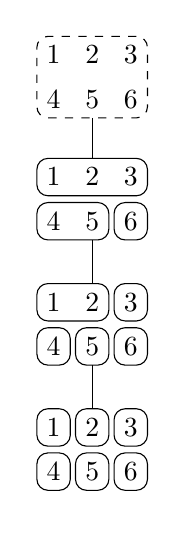
\begin{tikzpicture}[remember picture,rotate=0,
			group/.style={fill opacity=.2, inner sep=0, outer sep=0, rounded corners},
			every node/.style={rounded corners, text opacity=1, transform shape}
			]
			\def\position{below}
			\matrix(p0)at(0,0)[matrix of math nodes, ampersand replacement=\&,
			row sep=1mm,
			column sep=.8mm,
			every cell/.style={anchor=base west}]{
				1 \& 2\& 3 \\
				4 \& 5\& 6 \\
				\\};
			\def\dist{1.8}
			\def\distx{.3cm}
			\def\disty{.2cm}
			%
			\matrix(p1) [\position = 0.9*\disty of p0,
			matrix of math nodes, ampersand replacement=\&,
			row sep=1mm,
			column sep=.8mm,
			every cell/.style={anchor=base west}]{
				1 \& 2\& 3 \\
				4 \& 5\& 6 \\
				\\};
			\matrix(p2)[\position = 1.1*\disty of p1,
			matrix of math nodes, ampersand replacement=\&,
			row sep=1mm,
			column sep=.8mm,
			every cell/.style={anchor=base west}]{
				1 \& 2\& 3 \\
				4 \& 5\& 6 \\
				\\};
			\matrix(p3)[\position = 1.1*\disty of p2,
			matrix of math nodes, ampersand replacement=\&,
			row sep=1mm,
			column sep=.8mm,
			every cell/.style={anchor=base west}]{
				1 \& 2\& 3 \\
				4 \& 5\& 6 \\
				\\};
			% clustering of Z in PLP
			\node(p0)[dashed, draw, group, fill=none, fit=(p0-1-1)(p0-2-3)]{};
			%
			\node[draw, \thickness, group, fill=none, fit=(p1-1-1)(p1-1-3)]{};
			\node[draw, \thickness, group, fill=none, fit=(p1-2-1)(p1-2-2)]{};
			\node[draw, group, fill=none, fit=(p1-2-3)(p1-2-3)]{};
			\node(p1)[group, fill=none, fit=(p1-1-1)(p1-2-3)]{};
			%
			\node[draw, group, \thickness, fill=none, fit=(p2-1-1)(p2-1-2)]{}; \node[draw, group, fill=none, fit=(p2-1-3)]{};
			\node[draw, group, fill=none, fit=(p2-2-1)]{};
			\node[draw, group, fill=none, fit=(p2-2-2)]{};
			\node[draw, group, fill=none, fit=(p2-2-3)]{};
			\node(p2)[group, fill=none, fit=(p2-1-1)(p2-2-3)]{};
			%
			\node[draw, group, fill=none, fit=(p3-1-1)]{};
			\node[draw, group, fill=none, fit=(p3-1-2)]{};
			\node[draw, group, fill=none, fit=(p3-1-3)]{};
			\node[draw, group, fill=none, fit=(p3-2-1)]{};
			\node[draw, group, fill=none, fit=(p3-2-2)]{};
			\node[draw, group, fill=none, fit=(p3-2-3)]{};
			\node(p3)[group, fill=none, fit=(p3-1-1)(p3-2-3)]{};
			%%%%%%%%%%%%%%%%%%%%%%%%%%%%%%%%%%%%%%%%%%%
			%
			%
			%	% clustering of Z in PLP
			%
			%	\node[draw, group, fill=none, fit=(p3-1-1)]{};
			%	\node[draw, group, fill=none, fit=(p3-1-2)]{};
			%	\node[draw, group, fill=none, fit=(p3-1-3)]{};
			%	\node[draw, group, fill=none, fit=(p3-2-1)]{};
			%	\node[draw, group, fill=none, fit=(p3-2-2)]{};
			%	\node[draw, group, fill=none, fit=(p3-2-3)]{};
			%	%
			\draw(p0)--(p1)--(p2)--(p3);
%			\draw[dashed,overlay] (1)--(p0.east|-1);	
%			\draw[dashed,overlay] (2)--(p0.east|-2);
%			\draw[dashed,overlay] (3)--(p0.east|-3);
			\end{tikzpicture}
%		}\hfill
%	\end{center}
%	\caption{Dilworth truncation}
%\label{fig:eg-dt}
%\end{figure}

		}
		}%
		%\hfill
		%%%%%%%%%%%%%%%%%%%%%%%%
		\subcaptionbox{ \label{fig:eg-div-zv}}{
		\def\thickness{very thick}
		\scalebox{0.8}{
					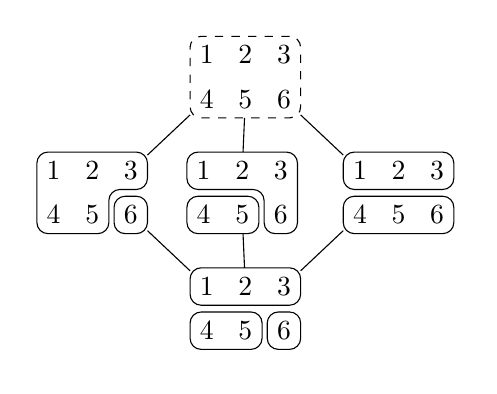
\begin{tikzpicture}[
		group/.style={fill opacity=.2, inner sep=0, outer sep=0, rounded corners},
		every node/.style={rounded corners, text opacity=1, fill opacity=.2}
		]
		
		
		\matrix(p0)at(2,-2)[matrix of math nodes, ampersand replacement=\&,
		row sep=1mm,
		column sep=.8mm,
		every cell/.style={anchor=base west}]{
			1 \& 2\& 3 \\
			4 \& 5\& 6 \\
			\\};
		\def\dist{1.8}
		\def\distx{.3cm}
		\def\disty{.1cm}
		\matrix(pl0)[below left = \disty and \distx of p0,
		matrix of math nodes, ampersand replacement=\&,
		row sep=1mm,
		column sep=.8mm,
		every cell/.style={anchor=base west}]{
			1 \& 2\& 3 \\
			4 \& 5\& 6 \\
			\\};
		\matrix(pm0)[below = \disty of p0,
		matrix of math nodes, ampersand replacement=\&,
		row sep=1mm,
		column sep=.8mm,
		every cell/.style={anchor=base west}]{
			1 \& 2\& 3\& \\
			4 \& 5\& 6\& \\
			\\};
		\matrix(pr0)[below right = \disty and \distx of p0,
		matrix of math nodes, ampersand replacement=\&,
		row sep=1mm,
		column sep=.8mm,
		every cell/.style={anchor=base west}]{
			1 \& 2\& 3\& \\
			4 \& 5\& 6\& \\
			\\};
		\matrix(p1)[below = \disty of pm0,
		matrix of math nodes, ampersand replacement=\&,
		row sep=1mm,
		column sep=.8mm,
		every cell/.style={anchor=base west}]{
			1 \& 2\& 3 \\
			4 \& 5\& 6 \\
			\\};
		
		% clustering of Z in PLP
		\node[dashed, draw, group, fill=none, fit=(p0-1-1)(p0-2-3)]{};
		%			%
		\node(pp0)[draw, group, fill=none, fit=(pl0-2-3)]{};
		\draw[rounded corners](pl0-1-1.north west)--(pl0-1-3.north east)--(pl0-1-3.south
		east)--(pl0-1-2.south east)--(pl0-2-2.south east)--(pl0-2-1.south west)-- cycle;
		%			%
		\node(pp0)[draw, group, fill=none, fit=(pm0-2-1)(pm0-2-2)]{};
		\draw[rounded corners](pm0-1-1.north west)--(pm0-1-3.north east)--(pm0-2-3.south east)
		--(pm0-2-3.south west)--(pm0-1-3.south west)--(pm0-1-1.south west)-- cycle;
		%			%
		\node[draw, group, fill=none, fit=(pr0-1-1)(pr0-1-3)]{};
		\node[draw, group, fill=none, fit=(pr0-2-1)(pr0-2-3)]{};
		%			%
		\draw(p0-2-1)--(pl0-1-3);
		\draw(p0-2-2)--(pm0-1-2);
		\draw(p0-2-3)--(pr0-1-1);
		%			%
		\draw(p1-1-1)--(pl0-2-3);
		\draw(p1-1-2)--(pm0-2-2);
		\draw(p1-1-3)--(pr0-2-1);
		%
		\node(pp0)[draw, \thickness, group, fill=none, fit=(p1-1-1)(p1-1-3)]{};
		\node(pp0)[draw, \thickness, group, fill=none, fit=(p1-2-1)(p1-2-2)]{};
		\node(pp0)[draw, group, fill=none, fit=(p1-2-3)]{};
		%			%
		\end{tikzpicture}

		}
		}%\hfill
		\subcaptionbox{\label{fig:eg-div-z123}}{
			\def\thickness{very thick}
			\scalebox{0.8}{
						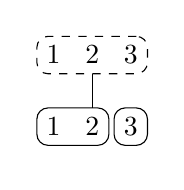
\begin{tikzpicture}[
			group/.style={fill opacity=.2, inner sep=0, outer sep=0, rounded corners},
			every node/.style={rounded corners, text opacity=1}
			]
			
			
			\matrix(p0)at(2,-2)[matrix of math nodes, ampersand replacement=\&,
			row sep=1mm,
			column sep=.8mm,
			every cell/.style={anchor=base west}]{
				1 \& 2\& 3 \\
				\\};
			\def\dist{1.8}
			\def\distx{.3cm}
			\def\disty{.1cm}
			\matrix(p1)[below = \disty of p0,
			matrix of math nodes, ampersand replacement=\&,
			row sep=1mm,
			column sep=.8mm,
			every cell/.style={anchor=base west}]{
				1 \& 2\& 3 \\
				\\};
			
			% clustering of Z in PLP
			\node[dashed, draw, group, fill=none, fit=(p0-1-1)(p0-1-3)]{};
			%			%
			\node[draw, \thickness, group, fill=none, fit=(p1-1-1)(p1-1-2)]{};
			\node[draw, group, fill=none, fit=(p1-1-3)]{};
			%			%
			\draw(p0-1-2)--(p1-1-2);
			\end{tikzpicture}

		}
		}%
%		\hfill
%		\subcaptionbox{$\mcP^{*}(\RZ_{\Set{4,5}})$ \label{fig:eg-div-z45}}[3cm]{
%			\input{dtl/dtl-45.tex}
%		}
	\end{center}
	\caption{
%		Optimal partitions of: (a) $I(\RZ_V)$ and (b) $I(\RZ_{\Set{1,2,3}})$. In each case, the
%		fundamental partition is the one at the bottom, where the associated clusters are circled with
%		thick lines.
		(a) The PSP of Example~\ref{eg:psp}, where the non-trivial clusters are circled with thick lines.  
		(b) and (c) Optimal partitions of $I(\RZ_V)$ and  $I(\RZ_{\Set{1,2,3}})$, respectively, of
		Example~\ref{eg:divisive}. In (b) and (c), the
		fundamental partition is the one at the bottom and the associated clusters are circled with
		thick lines.
	}
\label{fig:eg-div}
\end{figure}
%%%%%%%%%%%%%%%%%%%%%%%%%




%We end this section with a brief discussion on the Dilworth truncation and an equivalent
%characterization of the MMI to \eqref{eq:mmi}.
%\textcolor{red}{aaa-continue!}
%%%%%%%%%%%%%%
%The multivariate mutual information (MMI) is characterized in~\cite{chan15mi} as the
%smallest value of $`g\in `R$ such that the \emph{residual~independence relation (RIR)} holds, i.e.,
%for some partition $\mcP\in \Pi'(V)$,
%\begin{subequations}
%\begin{alignat}{2}
%	\label{eq:RIR}
%	h_{`g}(V) &= \sum_{C\in\mcP} h_{`g}[\mcP] &\kern1em& \text {where}\\
%	h(B)&:=H(\RZ_B) && \text{for } B\subseteq V, \label{eq:h}\\
%	h_{`g}(B)&:= h(B)-`g && \text{and} \label{eq:residualH}\\
%	h_{`g}[\mcP] &:= \sum\nolimits_{C\in \mcP} h_{`g}(C) && \text{for $\mcP\in \Pi (V)$}. \label{eq:DT:2} 
%\end{alignat}
%\end{subequations}
%Here, $h$ is the entropy function and $h_{`g}(B)$ is the \emph{residual entropy/randomness} of
%$\RZ_B$ after removing $`g$. The l.h.s.\ of \eqref{eq:RIR} is the total residual randomness of the
%entire set of random variables, and the r.h.s.\ is the sum of the individual residual randomness of
%a partition of the random variables. The equality means that there is independence (no double
%counting) in the individual residual randomness, i.e., $`g$ is the amount of mutual randomness whose
%removal leads to an independence relation.
%%%%%%%%%%%%%%%%%%%%%
%%More explicitly, the MMI, denoted as $I(\RZ_V)$, can equivalently be written as
%This characterization is equivalent to the followoing (explicit) formulation of the MMI, denoted as $I(\RZ_V)$, can be written as
%%%%%%%%%%%%%%

\section{Divisive approach}
\label{sec:divisive}

With the laminar structure in Proposition~\ref{prop:clusters}, a divisive algorithm was given in \cite{chan16cluster} to
compute $`g_\ell$ and $\mcP_{\ell}$ by iteratively producing finer partitions from coarser ones,
%i.e., from $\ell=1$ to $N$. 
i.e., from $\mcP_1$ to $\mcP_N$. 
The following result is instrumental in the devising of such an algorithm.
%
\begin{Proposition}[\mbox{\cite[Theorems~5.2 \& 5.3]{chan15mi}, \cite[Theorem~4]{chan16cluster}}]
	\label{prop:fund:cluster}
	The optimal partitions achieving the MMI in~\eqref{eq:mmi} together with the trivial partition $\{V\}$ form a
	lattice w.r.t.\ \eqref{eq:finer}. The minimum/finest optimal partition,
	%denoted  $\mcP^{*}(\RZ_V)$, satisfies 
	called the fundamental partition and denoted by $\mcP^{*}(\RZ_V)$, satisfies 
	\begin{align*}
		\mcP^{*}(\RZ_V) \backslash \{\{i\}\mid i\in V\} = \pzC_{I(\RZ_V)}(\RZ_V),
	\end{align*}
	with $\pzC_{`g}$ defined in \eqref{eq:clusters}.
	In other words,  $`g_1 = I(\RZ_V)$ and $\mcP_{1} = \mcP^{*}(\RZ_V)$ in
	Proposition~\ref{prop:clusters}. Finally, for $\ell \geq 1$,
	%if there exists $C \in \mcP_{\ell}:\abs {C}>1$,
	%if $\mcP_{\ell}$ is not the singletons partition,
	if $\mcP_l$ is not the partition into singletons,
	then $`g_{\ell +1} = \min\nolimits_{C\in \mcP_{\ell}:\abs{C}> 1}I(\RZ_C)$ and
	$\mcP_{\ell+1}\supseteq \mcP^*(\RZ_C)$ for any minimizer $C$.
\end{Proposition}
%Together with the laminar structure in Proposition~\ref{prop:clusters}, it can be argued that 
Because of the last statement in the proposition, any algorithm for computing $\mcP^{*}(\RZ_V)$ can
be applied iteratively for the divisive info-clustering approach as in~\cite[Algorithm~2]{chan16cluster}.
However,
as discussed near the end of~Section~\ref{sec:introduction},
this divisive approach can be a factor $n$ slower than \cite[Algorithm~3]{chan16cluster}.

\begin{example}
	\label{eg:divisive}
	As an illustration of Proposition~\ref{prop:fund:cluster} and the divisive approach, consider
	$\RZ_{\{1,\dots,6\}}$ in \eqref{eq:eg-motivate}.
%%%%%%%%%%%%%%%%%%%%%%%%%%%%%%%%%%%%%%%%%
	The finest optimal partition
	$\mcP^{*}(\RZ_V) = \Set{\Set{1,2,3},\Set{4,5},\Set{6}}$ is shown in \figref{fig:eg-div-zv}, and
	so one can easily verify from \eqref{eq:I} that $I(\RZ_{V}) = 0$.
	For completion, the figure also shows the lattice of optimal partitions stated in the proposition,
	where the trivial partition $\Set{V}$ is indicated using a dashed line.
	Similarly, \figref{fig:eg-div-z123} shows the optimal partitions of
	$\RZ_{\Set{1,2,3}}$.
	Since $I(\RZ_{V}) = 0$, Proposition~\ref{prop:fund:cluster}
	asserts that $\pzC_{0}(\RZ_V) = \Set{\Set{1,2,3},\Set{4,5}}$.
	Since $I(\RZ_{\Set{1,2,3}}) =I(\RZ_{\Set{4,5}})=1$ (and $\Set{1,2,3}$
	is the only cluster
	%among the two whose finest optimal partition is not the partition into singletons),
	%whose finest optimal partition contains a non-singleton),
	with a non-singleton in its finest optimal partition),
	Proposition~\ref{prop:fund:cluster} asserts that
	$\pzC_{1}(\RZ_V)=\pzC_1(\RZ_{\Set {1,2,3}}) = \Set{\Set{1,2}}$. 

%%%%%%%%%%%%%%%%%%%%%%%%%%%%%%%%%%%%%%%%%
%	Assuming an algorithm for computing the
%	finest optimal partition, the divisive algorithm starts by computing 
%	$\mcP^{*}(\RZ_V) = \Set{\Set{1,2,3},\Set{4,5},\Set{6}}$ (from which $I(\RZ_V)$ is readily
%	available), declares the non-singleton elements as clusters at threshold $I(\RZ_V)$,
%	and proceeds iteratively by picking any cluster (of size larger than two) and computing its
%	finest optimal partition, etc. In our example, there are two clusters, the sets $\Set{1,2,3}$ and $\Set{4,5}$
%	at threshold $0$.
%%	The finest optimal partition of $\RZ_{\Set{1,2,3}}$ is shown in
%%	Fig.~\ref{fig:eg-div-z123}, which results in the cluster $\Set{1,2}$ at threshold
%%	$I(\RZ_{\Set{1,2,3}}) = 1$.
%%	Also, $I(\RZ_{\Set{4,5}}) = 1$ with $\mcP^{*}(\RZ_{\Set{4,5}}) = \Set{\Set{4},\Set{5}}$.
%	%
%	At threshold $I(\RZ_{\Set{1,2,3}}) = 1$, $\Set{1,2,3}$ results in the cluster $\Set{1,2}$ since this is only nonsinglton element of $\mcP^{*}(\RZ_{\Set{1,2,3}})$ as shown in Fig.~\ref{fig:eg-div-z123}.
%	At threshold $I(\RZ_{\Set{4,5}}) = 1$, $\Set{4,5}$ gives no clusters since $\mcP^{*}(\RZ_{\Set{4,5}}) = \Set{\Set{4},\Set{5}}$.
%	At threshold $I(\RZ_{\Set{1,2}}) = 2$, $\Set{1,2}$ gives no clusters since $\mcP^{*}(\RZ_{\Set{1,2}}) = \Set{\Set{1},\Set{2}}$.
%	After this, the algorithm terminates with the entire hierarchy of clusters as in \eqref{eq:eg-clusters}.
%	%
	Assuming an algorithm for computing the
	finest optimal partition, the divisive algorithm starts by computing 
	$\mcP^{*}(\RZ_V) = \Set{\Set{1,2,3},\Set{4,5},\Set{6}}$ (from which $I(\RZ_V)$ is readily
	available), declares the non-singleton elements as clusters at threshold $I(\RZ_V)$,
	and proceeds iteratively by picking any cluster (of size larger than two) and computing its
	finest optimal partition, etc.
	In our example, $\mcP^{*}(\RZ_V)$ is shown in Fig.~\ref{fig:eg-div-zv}, which results in the clusters $\Set{\Set{1,2,3}, \Set{4,5}}$ at threshold $I(\RZ_{V}) = 0$.
	Next, $\mcP^{*}(\RZ_{\Set{1,2,3}})$ is shown in Fig.~\ref{fig:eg-div-z123}, which results in the cluster $\Set{1,2}$ at threshold $I(\RZ_{\Set{1,2,3}}) = 1$.
	%$\mcP^{*}(\RZ_{\Set{4,5}}) = \Set{\Set{4},\Set{5}}$, which procudces no clusters at threshold $I(\RZ_{\Set{4,5}}) = 1$.
	%$\mcP^{*}(\RZ_{\Set{1,2}}) = \Set{\Set{1},\Set{2}}$, which prodices no clusters at threshold $I(\RZ_{\Set{1,2}}) = 2$.
	After this, the divisive algorithm terminates with the entire hierarchy of clusters as in \eqref{eq:eg-clusters}.
	(In this example, the algorithm did not compute the last threshold in \eqref{eq:eg-clusters}, but it can do
	so by letting it proceed to clusters of size two.)
\end{example}
%%%%%%%%%%%%%%%%%%%%%%%%%%%%%%%%%

%The divisive approach can be a factor $n$ slower than \cite[Algorithm~3]{chan16cluster} as discussed in Section~\ref{sec:complextiy}.
%The divisive approach can be a factor $n$ slower than \cite[Algorithm~3]{chan16cluster} that
%computes (in no particular order) all the clusters. %Nevertheless, in practice it is desirable to have 
%Nevertheless, an iterative approach of computing the clusters in order remains desirable
%in practice as it can stop when further computations are not of
%interest or are meaningless due to errors in estimating the entropies from data.
%Agglomerative info-clustering will achieve this appealing iterative computation (according to order)
%while retaining the same run-time complexity as \cite[Algorithm~3]{chan16cluster}. 





\section{Principal sequence and minimum norm base}
\label{sec:prelim}
%\input{prelim}


%The ability to compute the info-clustering solution efficiently stems from the submodularity of
%entropy~\cite{fujishige78}, or equivalently the fact that conditional mutual information is
%non-negative~\cite{shannon48}. More precisely,
%the \emph{submodularity} of entropy means that the entropy function $h$ in \eqref{eq:h} satisfies
%\begin{align}
%	h(B_1)+h(B_2)\geq h(B_1\cup B_2)+h(B_1\cap B_2)  \label{eq:submodular}
%\end{align}
%for all $B_1,B_2\subseteq V$.
%The entropy function is also said to be \emph{normalized} since $h(`0)=0$, and non-decreasing since $h(B')\leq h(B)$ whenever $B' \subseteq B \subseteq V$.
%In combinatorial optimization~\cite{schrijver02}, submodularity is well-known to often give rise to polynomial-time solutions. 
As discussed earlier, the PSP of $h$ is polynomial time solvable, which
characterizes the info-clustering solution by Proposition~\ref{prop:clusters}.
Our agglomerative algorithm
will make use of yet another polynomial time solvable structure, discussed below,
that is closely related to the PSP.
% as explained in Section~\ref{sec:results}.
%The details may be skipped for the first reading.


Consider any submodular function $f:2^U\to `R$~\eqref{eq:submodular} on the finite ground set $U$. For $`l\in `R$, define
\begin{align}
\kern-.5em S_{`l}(f):=\max \argmin_{B\subseteq U} f(B)-`l\abs{B}, \label{eq:S_`l}
\end{align}
where $\max$ is the inclusion-wise maximum.
Note that the minimization in \eqref{eq:S_`l} is a \emph{submodular function minimization (SFM)}
since the function $B\subseteq U\mapsto f(B)-`l\abs{B}$ is also submodular. It is well-known that
the minimizers of a submodular function form a lattice w.r.t. set inclusion~\cite{schrijver02}, and so the maximum
in \eqref{eq:S_`l} exists and is unique.  
\begin{Proposition}[\mbox{\cite{fujishige80,fujishige-pp-revisited}}] 
	\label{prop:ps}
	$S_{`l}(f)$ for $`l\in`R$ satisfies
	 \begin{align*}
		 \label{eq:aaa-ps}
	 	S_{`l'}(f)\subseteq S_{`l''}(f) \kern1em \text {iff} \kern1em `l'\leq `l''.
	 \end{align*}
%	 %and is referred to as the principal sequence (PS).
	 This defines a  sequence, for some positive integer $N'$, 
	 \begin{align}
		 \label{eq:aaa-pss}
		 S_{\lambda_{0}} := \emptyset \subsetneq S_{\lambda_1} \subsetneq \dots \subsetneq S_{\lambda_{N'-1}} \subsetneq S_{\lambda_{N'}} := V
	 \end{align}
	 of distinct sets, which
	 (together with the sequence $-\infty = \lambda_{0} < \lambda_1 < \dots < \lambda_{N'} <
	 \lambda_{N'+1} := \infty$ of $\lambda$ values at which $S_{\lambda}$ changes)
	 is referred to as the principal sequence (PS).
%%	 The sequence 
%%	 \begin{align*}
%%		 S_{\lambda_{0}} := \emptyset \subsetneq S_{\lambda_1} \subsetneq \dots \subsetneq S_{\lambda_{N'-1}} \subsetneq S_{\lambda_{N'}} := V
%%	 \end{align*}
%%	 of distinct sets
%%	 (together with the sequence $-\infty = \lambda_{0} < \lambda_1 < \dots < \lambda_{N'} < \lambda_{N'+1} := \infty$)
%%	 is referred to as the principal sequence (PS).
\end{Proposition}
%$S_{`l}(f)$ can be characterized and computed in strongly polynomial time as follows:
%	Equation \eqref{eq:aaa-ps} defines a  sequence, for some positive integer $N'$, 
%	 \begin{align*}
%		 S_{\lambda_{0}} := \emptyset \subsetneq S_{\lambda_1} \subsetneq \dots \subsetneq S_{\lambda_{N'-1}} \subsetneq S_{\lambda_{N'}} := V
%	 \end{align*}
%	 of distinct sets. This sequence
%	 (together with the sequence $-\infty = \lambda_{0} < \lambda_1 < \dots < \lambda_{N'} <
%	 \lambda_{N'+1} := \infty$ of $\lambda$ values at which $S_{\lambda}$ changes)
%	 is referred to as the principal sequence (PS).

W.l.o.g., we assume $f$ is normalized, i.e., $f(`0)=0$, since we can redefine
$f$ as $f-f(`0)$ without  affecting the solutions to the SFM in~\eqref{eq:S_`l}, i.e., aside from a
shift in the $\lambda_i$ values, the
PS~\eqref{eq:aaa-pss} is
invariant to a constant shift in the submodular function. The polyhedron $\rmP(f)$ and base polyhedron
$\rmB(f)$ of the submodular function $f$ are defined as
\begin{subequations}
	\label{eq:PB}
\begin{align}
	\rmP(f)&:=\Set {x_U\in `R^U\mid x(B)\leq f(B),\forall B\subseteq U} \label{eq:rmP}\\
	\rmB(f)&:=\Set {x_U\in \rmP(f)\mid x(U)=f(U)}, \label{eq:rmB}
\end{align}
\end{subequations}
where $x_U:=(x_i\mid i\in U)$ and $x(B):=\sum_{i\in B} x_i$. (N.b., $\rmP(f)$ and
$\rmB(f)$ are non-empty since $f(`0)\geq 0$.) With $\norm {x_U}$ denoting the Euclidean norm of the
vector $x_U$, the following holds.

\begin{Proposition}[\mbox{\cite{fujishige80,fujishige11}}]
	\label{prop:MNB}
	For any normalized submodular function $f$~\eqref{eq:submodular},
	the minimization
	\begin{align}
		\label{eq:MNB}
		\min \Set{\norm{x_U}\mid x_U\in \rmB(f)}
		%\min_{x_{U}\in \mathbb{R}^{U} } \Set{\norm{x_U} \mid x_U \in \mathbb{R}^{U},  x(B)\leq f(B) \ \forall B\subseteq U, x(U) = f(U)}
	\end{align}
	has a unique solution $x_U^*$, called the minimum (Euclidean) norm base, which satisfies
	\begin{subequations}
	\begin{alignat}{2}
		\kern-1em x^*_i&=\min\Set{`l\in`R\mid i\in  S_{`l}(f)}&\kern1em& \forall i\in U, \text {or equiv.,}\label{eq:MNB:x*}\kern-.5em\\
		\kern-1em S_{`l}(f)&=\Set{i\in U\mid x^*_i\leq `l},&\kern1em & \forall `l\in `R,\label{eq:MNB:S_`l}
	\end{alignat}
	\end{subequations}
	where the equivalence follows directly from Proposition~\ref{prop:ps}.
\end{Proposition}

The minimum norm base, and so the PS by \eqref{eq:MNB:S_`l}, may be computed using Wolfe's minimum norm point algorithm as
in~\cite{fujishige11}. Conversely, by \eqref{eq:MNB:x*},
the minimum norm base can also be computed by any SFM algorithm that solves $S_{`l}$ for any $`l$.
However, the minimum norm point algorithm was shown~\cite{fujishige11} empirically to outperform other SFM algorithms. 




\section{Main results}
\label{sec:agglom}

Instead of the divisive approach, we consider here an agglomerative approach, 
%Algorithm~\ref{alg:aic}, that computes $`g_{\ell}$ and $\mcP_{\ell}$ iteratively from $\ell=N$
Algorithm~\ref{alg:aic}, that computes $`g_{\ell}$ and $\mcP_{\ell}$ by iteratively producing coarser partitions from finer ones, i.e., from $\mcP_N$ to $\mcP_1$. 
(Note that $N$ needs not be known a priori.)
%We will give an efficient implementation of the subroutine \Agglomerate in Algorithm~\ref{algo:fuse}
%that computes $`g_\ell$ and $\mcP_{\ell-1}$ from $\mcP_{\ell}$ for any $\ell$, hence resolving the
%inefficiency of the divisive approach while returning the clusters in order.  In particular, we will
%show that it suffices to compute
We will give an efficient implementation (thereby resolving the inefficiency of the divisive
approach) of the subroutine \Agglomerate in Algorithm~\ref{algo:fuse}, which computes $`g_\ell$ and
$\mcP_{\ell-1}$ from $\mcP_{\ell}$ for any $\ell$ (thereby returning the clusters in the desired order).
In particular, we will show that it suffices to compute
\begin{subequations}
	\label{eq:IC*}
\begin{align}
	I^*(\RZ_V)&:=\max\{I(\RZ_{C})\mid C\subseteq V, \abs {C} > 1\} \kern1em \text{ and}\label{eq:I*}\\
	\begin{split}
	\pzC^*(\RZ_V)&:=\op{maximal}\{C\subseteq V \mid \abs{C} > 1, \\
	&\kern8em I(\RZ_C) = I^{*}(\RZ_{V})  \},
	\end{split}\label{eq:C*}
\end{align}
\end{subequations}
which are, respectively, the last critical value $`g_{N}$  \cite[Theorem~1]{chan16cluster} and the last set of clusters (i.e., the non-singleton elements of the second last
partition $\mcP_{N-1}$).
%%%%%%%%%%%%%%%%%%%%%%%%%%%%%%%
%These quantities turn out to have a fundamental connection
%with the normalized total correlation~\eqref{eq:JT}, which gives rise to the efficient
%implementation.
%%%%%%%%%%%%%%%%%%%%%%%%%%%%%%
Recall 
%the MMI 
%as in~
\eqref{eq:I} 
and note that 
if the partition $\mcP=\Set {\Set {i}\mid i\in V}$ is
optimal
%to \eqref{eq:I},
then the MMI is equal to
\begin{align}
	\label{eq:JT}
	\begin{split}
		J_{\opT}(\RZ_V)
		&:=I_{\Set{\Set{i}\mid i\in V}}(\RZ_V)\\
		%&=\frac1 {\abs{V}-1}`1[\sum\nolimits_{i \in V}H(\RZ_i)-H(\RZ_V)`2],
		&=\frac1 {\abs{V}-1}`1[\sum\nolimits_{i \in V}h(\Set{i})-h(V)`2],
	\end{split}
\end{align}
which is the normalized version (see~\cite{chan15mi} for more details) of
the well-known Watanabe's total correlation~\cite{watanabe60}.
%%%%%%%%%%%%%%%%%%%%%%%%%%%%%%
The quantities $I^{*}$ and $\pzC^{*}$ turn out to have a fundamental connection
with the normalized total correlation~\eqref{eq:JT}, which leads to the desired efficient
implementation.


%\label{sec:results}
%\input{results}

%%%%%%%%%%%%%%%%%%%%%%%%%%%%%%%%%%%%%%%%%%%%%%%%%%%%%%
\begin{algorithm}
	\caption{Agglomerative info-clustering.}
	\label{alg:aic}
	\KwData{Statistics of $\RZ_V$ sufficient for calculating the entropy function $h(B)$ for
		$B\subseteq V:=\{1,\ldots,n\}$.}
	\KwResult{Two arrays \DataSty{L} and \DataSty{PSP} that contain the $`g_{\ell}$'s and $\mcP_{\ell}$'s
		in Proposition~\ref{prop:clusters}. More precisely,
		for $1\leq \ell \leq N$, the entries of the arrays
		\DataSty{L}
		and
		\DataSty{PSP}
		are 
		\DataSty{L}$[s] = `g_{\ell}$
		and
		\DataSty{PSP}$[s] = \mcP_{\ell}$
		for $s = |\mcP_{\ell}|$, 
		and are null otherwise.}
	\BlankLine
	\DataSty{L}, \DataSty{PSP}$\leftarrow$ empty arrays, each of length $n$;\;
	\DataSty{PSP}$[n]$ $\leftarrow \{\{i\}:i\in V\}$, $s\leftarrow n$;\;
	\While{$s>1$}{
		$(`g,\mcP')\leftarrow$ $\Agglomerate($\DataSty{PSP}$[s])$;\;
		\DataSty{L}$[s]\leftarrow `g$;
		$s\leftarrow |\mcP'|$;
		\DataSty{PSP}$[s]\leftarrow \mcP'$;\;
	}
	% 	\BlankLine
	%   	\myfn{\Agglomerate{$\mcP$}}{
	%			assume $\mcP=\mcP_{\ell}$ for $1\leq \ell\leq N$ in Proposition~\ref{prop:clusters};\;
	%			\KwRet $(`g,\mcP_{\ell}) \leftarrow (`g_{\ell},\mcP_{\ell-1})$;
	%   	}
	%	\textcolor{red}{---needs revision, particularly the function fuse.}
\end{algorithm}
%%%%%%%%%%%%%%%%%%%%%%%%%%%%%%%%%%%%%%%%%%%%%%%%%%%%%%

The main result is the implementation of \Agglomerate in Algorithm~\ref{algo:fuse} that computes the
PSP, and so the info-clustering solution, iteratively from finer partitions to coarser
ones. This is done by computing the PS using a subroutine \MinNormBase that computes the minimum
norm base for \eqref{eq:MNB}. An explicit implementation of \MinNormBase can be found in
\cite{fujishige11} using Wolfe's minimum norm point algorithm.
%The current abstraction also allows further approximations or simplifications for special source models as in \cite{chan16cluster}. 

\begin{algorithm}
	\caption{Implementation of \texttt{agglomerate}.}% in Algorithm~\ref{alg:aic}.}
	\label{algo:fuse}
	%	\KwData{Statistics of $\RZ_V$ sufficient for calculating \FirstClusters{$B$} for all $B\subseteq V:\abs{B}>1$.}
	%	\KwResult{$\mcS$ is a list of $(I(\RZ_C),C)$ for $C\in \pzC(\RZ_V)$, which gives
	%		$\Upgamma(\RZ_V)=\Set{`g' \mid (`g',B)\in \mcS}$ and
	%		$\pzC_{`g}(\RZ_V)=\op{maximal}\Set{B\mid (`g',B)\in \mcS,`g'>`g}$.}
	%	\BlankLine
	\BlankLine
	\KwData{$\mcP$ is equal to $\mcP_{\ell}$ for some $1\leq \ell\leq N$ in \eqref{eq:PSP}.} %Proposition~\ref{prop:clusters}.}
	\KwResult{$(`g,\mcP')$ is equal to $(`g_\ell,\mcP_{\ell-1})$.}
	%\myfn{\Agglomerate{$\mcP$}}{
		Enumerate $\mcP$ as $\Set{C_1,\dots,C_k}$ for some $k>1$ and disjoint $C_i$'s;\;
		\DataSty{x}$\leftarrow$ empty array of size $k$;\;
		\For{$j\leftarrow 1$ \emph{\KwTo} $k$ }{
			%\DataSty{x}[$j$]=\MinNormBase($ B\mapsto h`1(\bigcup_{i\in B\cup\Set{j}}C_i`2)-\sum_{i\in B\cup\Set{j}}h(C_i),\Set{j+1,\ldots,k}$);\; \label{ln:MNB:1}
			Define $g_j$ as the function $ B\subseteq \{j+1,\dots,k\}  \mapsto h`1(\bigcup_{i\in B\cup\Set{j}}C_i`2)-\sum_{i\in B\cup\Set{j}}h(C_i)$;\; 
			\DataSty{x}[$j$]$\leftarrow$\MinNormBase($g_j,\Set{j+1,\ldots,k}$);\; \label{ln:MNB:1}
		}
		%\KwRet $(\upgamma_1(\RZ_B),\pzC_{\upgamma_1}(\RZ_B))$;
		$\displaystyle`g\leftarrow -\min_{i,j:1\leq j<i\leq k}\DataSty{x}[j][i]$,\kern1em$\mcP'\leftarrow`0$;\;
		\For{$j \leftarrow 1$ \emph{\KwTo} $k$ }{
			\If{$C_j\nsubseteq \bigcup\mcP'$}{
				%add $\Set{C_j}\cup\Set{C_i\mid i\kern-.25em\in\kern-.25em\Set{j\kern-.25em +\kern-.25em 1,\dots,k}, \DataSty{x}[j][i]\kern-.25em\leq\kern-.25em -`g}$ to $\mcP'$;\;
				add $C_j \cup \bigcup\Set{C_i\mid i\kern-.25em\in\kern-.25em\Set{j\kern-.25em
				+\kern-.25em 1,\dots,k}, \DataSty{x}[j][i]\kern-.25em\leq\kern-.25em -`g}$ to $\mcP'$;\;
				%\tcc{see below \eqref{} for the notation ``$\bigcup$''}
			}
%			\If{$C_j\not\in \bigcup_{C\in \mcP'}C'$}{
%				add $\Set{C_j}\cup\Set{C_i\mid i\kern-.25em\in\kern-.25em\Set{j\kern-.25em +\kern-.25em 1,\dots,k}, \DataSty{x}[j][i]\kern-.25em\leq\kern-.25em -`g}$ to $\mcP'$;\;
%			}
			
		}
		
	%}
	\myfn{\MinNormBase($f,U$)}{
		%\tcc{ assume normalized submodular function $f:2^U\mapsto`R$ }
		\KwRet an array \DataSty{x} (indexed by $U$) that solves~\eqref{eq:MNB}.
	}
\end{algorithm}

%%%%%%%%%%%%%%%%%%%%%%%%%%%%%
%
%The complexity of the algorithm is mainly due to the computation of the minimum norm base in
%line~\ref{ln:MNB:1}.
%%The number of such computation is at most $n$.
%This computation is repeated at most $n$ times.
%With $\op{MNB}(n)$ being
%the complexity of the minimum norm base algorithm for ground set of size $n$, \Agglomerate runs in
%time $O(n\op{MNB}(n))$. Since the agglomerative info-clustering algorithm in
%Algorithm~\ref{alg:aic} invokes function \Agglomerate $N-1\leq n-1$ times, it runs in time
%$O(n^2 \op{MNB}(n))$, which is equivalent to that of~\cite[Algorithm~3]{chan16cluster},
%assuming that the submodular function minimization therein is implemented by the minimum norm base
%algorithm, i.e., with $\op{SFM}=\op{MNB}$. The divisive info-clustering algorithm
%in~\cite[Algorithm~2]{chan16cluster} makes $N-1$ calls to a subroutine that calculates the
%fundamental partition. However, computing the fundamental partition appears to take time
%$O(n^2 \op{MNB}(n))$, which would lead to an overall complexity of $O(n^3
%\op{MNB}(n))$ for the divisible clustering. Hence, the agglomerative info-clustering is
%more efficient.
%
%%%%%%%%%%%%%%%%%%%%%%%%%%%%%

To explain Algorithm~\ref{algo:fuse}, we need the following two results that
\begin{inparaenum}
\item 
relate the last critical value of a set of RVs to the normalized total correlation and,
%as a result,
consequently,
to the minimum norm base; and
\item 
relate any critical value of a set of RVs to the last critical value of a set of agglomerated RVs.
\end{inparaenum}
Each theorem will be illustrated with an example. %that is followed by a proof sketch.
The statements of the results may be
skimmed first and read more carefully as we go through the examples.
%The detailed proofs can be found in~\cite{chan17aic}.

\begin{Theorem}
	\label{thm:JT}
	With $V:= \{1,\ldots, n\}$ and $h$ denoting the entropy function of $\RZ_V$, let,
	for any $j\in V$,
	\begin{align*}
		U_j &:=\Set {i\in V\mid i>j} \kern0em \text{ and } \\ %\text{ assuming $V$ is ordered.}\\
	g_j(B) &:= h(B\cup \Set {j})-\sum\nolimits_{i\in B\cup \Set {j}} h(\Set {i}) \kern1em \text {for }B\subseteq U_j,
	\end{align*}
	which is a normalized submodular function. Then,
	\begin{subequations}
		\begin{align}
		I^*(\RZ_V)&=\max_{C\subseteq V:\abs{C}> 1} J_{T}(\RZ_C) \label{eq:maxJT}\\
		&= -\min_{j\in V} \min_{i\in U_j} x^{(j)}_i \label{eq:maxJT:x}\\ \nextParentEquation
		\pzC^*(\RZ_V)&=\op{maximal}
		\argmax_{C\subseteq V:\abs{C}> 1} J_{T}(\RZ_C)
		\label{eq:argmaxJT}\\
		&=\op{maximal} 
		`1\{`1.\Set{j^*}\cup 
		\argmin_{i\in U_{j^*}} x^{(j^*)}_i `2|`2.  \notag\\
		&\kern6.5em 
		`1.j^*\in \argmin_{j\in V} `1( \min_{i\in U_{j}} x^{(j)}_i `2)
		`2\},\label{eq:argmaxJT:x}
		\end{align}
	\end{subequations}
	where $x^{(j)}_{U_{j}}$ is the minimum norm base for $g_j$~\eqref{eq:MNB}.
\end{Theorem}
\begin{Proof}
	See Appendix~\ref{sec:proof}.
\end{Proof}

\begin{example}
	\label{eg:IC*}
	%As an illustration of Theorem~\ref{thm:JT}, 
	Consider our running example~\eqref{eq:eg-motivate}
	with $V = \Set{1,\ldots,6}$. By brute-force search, the maximum normalized total correlation in
	\eqref{eq:maxJT} is $J_{\opT}(\RZ_{\Set {1,2}})=2$ achieved uniquely by $C=\Set {1,2}$. Hence,
	\eqref{eq:maxJT} and \eqref{eq:argmaxJT} give, respectively, $I^*(\RZ_V)=2$ and $\pzC^*(\RZ_V)=\Set {\Set
		{1,2}}$, which correspond to the last critical value and last set of clusters
		in \eqref{eq:eg-clusters}, as desired by the definitions of $I^*$ and $\pzC^*$ in
		\eqref{eq:IC*}. 
	
	To illustrate \eqref{eq:maxJT:x} and \eqref{eq:argmaxJT:x},  
	the minimum norm base $x_{U_{j}}^{(j)}$ of $g_{j}$, for different values of $j$, is calculated as:
	\begin{align*}
	x_{U_j}^{(j)} =
	\scalebox{0.8}{
		\begin{blockarray}{lcc ccl c}
		\phantom{n}1 &	2 & 3 & 4 & 5 & 6 \\
		\begin{block}{\{lcc ccc c}
		(&	\circled{-2}, & -1, & -0.5, & -0.5, & 0),   & j=1 \\
		(&	   & -1,  & -0.5, & -0.5, & 0),   & j=2 \\
		(&	   &      & -0.5, & -0.5, & 0),   & j=3 \\
		(&	   &      &      & -1,   & 0),   & j=4 \\
		(&	   &      &      &      & 0),   & j=5. \\
		\end{block}
		\end{blockarray}}
	\end{align*}
%	For instance, when $j=4$, we have $U_j=\Set {5,6}$, $g_j(`0)=h(\Set {j})-h(\Set {j})=0$ and
%	$g_j(\Set {5})=h(\Set {4,5})-h(\Set {4})-h(\Set {5})=-I(\RZ_4\wedge \RZ_5)=-1$. Similarly,
%	$g_j(\Set {6})=-I(\RZ_4\wedge \RZ_6)=0$. $g_j(\Set {5,6})=h(\Set {4,5,6})-h(\Set {4})-h(\Set
%	{5})-h(\Set {6})=-1$. From \eqref{eq:PB}, $\rmP(g_j)=\Set {(x_5,x_6)\in `R^2\mid x_5\leq -1,
%	x_6\leq 0}$ and so $\rmB(g_j)=\Set {(-1,0)}$ contains a unique base, which is  therefore the
%	minimum norm base trivially. 
%%
%	For instance, when $j=4$, we have $U_j=\Set {5,6}$ and $g_j(`0)=0$,
%	$g_j(\Set {5})=h(\Set {4,5})-h(\Set {4})-h(\Set {5})=-I(\RZ_4\wedge \RZ_5)=-1$,
%	$g_j(\Set {6})=-I(\RZ_4\wedge \RZ_6)=0$, and $g_j(\Set {5,6})=h(\Set {4,5,6})-h(\Set {4})-h(\Set
%	{5})-h(\Set {6})=-1$. From \eqref{eq:PB}, $\rmP(g_j)=\Set {(x_5,x_6)\in `R^2\mid x_5\leq -1,
%	x_6\leq 0}$, and so $\rmB(g_j)=\Set {(-1,0)}$ contains a unique base, which is  therefore the
%	minimum norm base trivially. 
%	
	Now, the minimum in \eqref{eq:maxJT:x} is equal to $-2$ (circled above), which is achieved uniquely by $j=1$ and $i=2$. This gives $I^*(\RZ_V)=-(-2)=2$ as desired. In \eqref{eq:argmaxJT:x}, we have $j^*\in \Set {1}$ and $\argmin_{i\in U_{j^*}} x_i^{(j^*)}=\Set {2}$. Hence, $\pzC^*(\RZ_V)=\op{maximal}\Set {\Set {1}\cup \Set {2}}=\Set {\Set {1,2}}$ as desired.	
	%
\end{example}


We remark that \eqref{eq:maxJT} and~\eqref{eq:argmaxJT} eliminate the need for minimization over
partitions in calculating the MMI in~\eqref{eq:I*} and~\eqref{eq:C*}. They serve as an intermediate
step that leads to \eqref{eq:maxJT:x} and \eqref{eq:argmaxJT:x},
thereby relating the last critical value
%\eqref{eq:I*}
and last set of clusters 
%\eqref{eq:C*}
to the minimum norm base. 

%\begin{Proof}[Sketch for Theorem~\ref{thm:JT}]
%	
%\eqref{eq:maxJT} and \eqref{eq:argmaxJT} can be proved by showing that the optimal partition for any
%maximizer $C$ to \eqref{eq:I*}  is the partition $\Set {\Set {i}\mid i\in C}$ into singletons, in
%which case $I(\RZ_C)=J_{\opT}(\RZ_C)$. 
%%\eqref{eq:maxJT} and \eqref{eq:argmaxJT} can be proved by showing that,
%%for any maximizer $C$ to \eqref{eq:I*}, 
%%the optimal partition achieving $I(\RZ_{C})$
%%is the partition $\Set {\Set {i}\mid i\in C}$ into singletons, and so $I(\RZ_C)=J_{\opT}(\RZ_C)$. 
%
%To obtain the minimum norm base formulation in \eqref{eq:maxJT:x} and \eqref{eq:argmaxJT:x}, the
%important step is to rewrite \eqref{eq:maxJT} as
%%\begin{align*}
%%0&=\min_{C\subseteq V:\abs{C}>1}`g^*-J_{\op{T}}(\RZ_C)\\
%%&=\min_{C\subseteq V:\abs{C}>1}(\abs{C}-1)`g^*+h(C)-\sum_{i\in C}h(\Set{i})  \\
%%&=\min_{j\in V}\min_{B\subseteq U_j:\abs{B}\geq1} g_j(B)+`g^*\abs{B}.
%%\end{align*}
%\begin{align*}
%	0&=\min_{C\subseteq V:\abs{C}>1} \big[I^*(\RZ_V)-J_{\op{T}}(\RZ_C) \big]\\
%	&=\min_{C\subseteq V:\abs{C}>1} \big[(\abs{C}-1) I^*(\RZ_V)+h(C)-\sum_{i\in C}h(\Set{i}) \big]  \\
%	&=\min_{j\in V}\min_{B\subseteq U_j:\abs{B}\geq1} g_j(B)+I^*(\RZ_V)\abs{B}.
%\end{align*}
%In particular, the inner minimization can be cast as the minimization in \eqref{eq:S_`l} for the PS, and the solution via the minimum norm base in \eqref{eq:MNB:S_`l} gives \eqref{eq:maxJT:x} and \eqref{eq:argmaxJT:x}.
%\end{Proof}



So far we succeeded in posing the computation of the last critical value $I^{*}$ and
last set of clusters $\pzC^{*}$ as a minimum norm base problem.
However, our objective is to compute the entire clustering solution.
To complete the implementation of \Agglomerate, we need the following theorem which reduces
the computation of the clusters at any threshold to the computation of $I^*$ and $\pzC^*$ for some
agglomerated RVs.
%, we have the complete implementation of \Agglomerate as shown in Algorithm~\ref{algo:fuse} using a minimum norm base algorithm.

%%%%%%%%%%%%%%%%%%%%%%%%%%%%%%%%%%%%%%%%%%%%%%%%%%%%%%%%%%%%%%%%%%%%%%%%%%
\begin{Theorem}
	\label{thm:`g:P:fused}
 Consider  $\mcP_{\ell}$ and $`g_\ell$ as defined in Proposition~\ref{prop:clusters} and, for $1\leq
 \ell\leq N$, write
 \begin{align}
 	\mcP_{\ell}=\Set{C_j\mid j\in U} \kern1em \text{and}\kern1em
 	\RZ'_j:=\RZ_{C_j} \label {eq:Z'}
 \end{align}
 for some index set $U$ and disjoint subsets $C_j$ for $j\in U$. Then, for $1\leq \ell \leq N$, we
 have
 \begin{subequations}[eq:A:`g]
 	\begin{align}
 	`g_\ell
	&=\max_{\mcF\subseteq \mcP_{\ell}:\abs{\mcF}>1} I(\RZ_{\bigcup \mcF}) \label{eq:A:`g_l}\\
 	&=I^*(\RZ'_U), %:=\max`1\{I(\RZ'_B)\mid B\subseteq U,\abs{B}>1`2\}
 	\label{eq:A:`g_l:fused}\\
 	\nextParentEquation[eq:A:P]
 	\kern-.7em\mcP_{\ell-1}`/\mcP_{\ell}
 	&=\op{maximal}\Set*{\bigcup\mcF`1| \mcF\in\kern-.5em \argmax_{\mcF\subseteq \mcP_{\ell}:\abs{\mcF}>1} \kern-.5em I(\RZ_{\bigcup \mcF}) \kern-.3em `2.}\kern-.5em\label{eq:A:P_i-1}\\
 	&=`1\{\bigcup\nolimits_{j\in B}C_j \mid B\in \pzC^*(\RZ'_U)`2\}, \label{eq:A:P_i-1:fused}
 	\end{align}
 \end{subequations}
where $\bigcup \mcF:=\bigcup_{B\in \mcF} B$ for convenience.
%More precisely, \eqref{eq:A:`g_l} and~\eqref{eq:A:P_i-1} follow more generally from the property~\eqref{eq:imunion}, while \eqref{eq:A:`g_l:fused} and \eqref{eq:A:P_i-1:fused} follow from 
%the definition~\eqref{eq:mmi} of the MMI.
\end{Theorem}
\begin{Proof}
	See Appendix~\ref{sec:proof}.
\end{Proof}
%%\newcommand{\cb}{\bigcup_{i\in B}C_i}
%%\newcommand{\cbb}{\bigcup\limits_{i\in B'}C_i}
%\newcommand{\cb}{C_B}
%\newcommand{\cbb}{C_{B'}}
%\begin{Theorem}
%	\label{thm:`g:P:fused}
% Consider $\mcP_{\ell}$ and $`g_\ell$ defined as in Proposition~\ref{prop:clusters} for $1\leq \ell\leq N$ and write
% \begin{align}
% 	\mcP_{\ell}=\Set{C_j\mid j\in U} \kern1em \text{and}\kern1em
% 	\RZ'_j:=\RZ_{C_j} \label {eq:Z'}
% \end{align}
% for some index set $U$ and disjoint subset $C_j$ for $j\in U$. Then, for $1\leq \ell \leq N$ we
% have
% \begin{subequations}[eq:A:`g]
% 	\begin{align}
%		`g_\ell&=\max_{B\subseteq U,\abs{B}>1} I(\RZ_{\cb}) \label{eq:A:`g_l}\\
% 	&=I^*(\RZ'_U)%:=\max`1\{I(\RZ'_B)\mid B\subseteq U,\abs{B}>1`2\}
% 	\label{eq:A:`g_l:fused}\\
% 	\nextParentEquation[eq:A:P]
% 	\kern-.7em\mcP_{\ell-1}`/\mcP_{\ell}
%	&=\op{maximal}\Set*{C_{B}`1| B\in\kern-.5em \argmax_{B'\subseteq U:\abs{B'}>1} \kern-.5em I(\RZ_{\cbb}) \kern-.3em `2.}\kern-.5em\label{eq:A:P_i-1}\\
%	&=`1\{\cb \mid B\in \pzC^*(\RZ'_U)`2\}, \label{eq:A:P_i-1:fused}
% 	\end{align}
% \end{subequations}
%where $C_B:=\bigcup_{i\in B} C_i$ for convenience.
%%More precisely, \eqref{eq:A:`g_l} and~\eqref{eq:A:P_i-1} follow more generally from the property~\eqref{eq:imunion}, while \eqref{eq:A:`g_l:fused} and \eqref{eq:A:P_i-1:fused} follow from 
%%the definition~\eqref{eq:mmi} of the MMI.
%\end{Theorem}

%\begin{Proof}
%	See Appendix~\ref{sec:proof}.
%\end{Proof}
%%%%%%%%%%%%%%%%%%%%%%%%%%%%%%%%%%%%%%%%%%%%%%%%%%%%%%%%%%%%%%%%%%%%%%%%%%



%It follows from~\eqref{eq:A:`g_l:fused} and~\eqref{eq:A:P_i-1:fused} that it suffices to compute $I^*$~\eqref{eq:I*} and $\pzC^*$~\eqref{eq:C*}. This can be done using a minimum norm base algorithm as follows. Define
%\begin{align}
%\label{eq:JT}
%\begin{split}
%J_{\opT}(\RZ_V)&:=I_{\Set{\Set{i}\mid i\in V}}(\RZ_V)\\
%&=\frac1 {\abs{V}-1}`1[\sum_{i \in V}H(\RZ_i)-H(\RZ_V)`2],
%\end{split}
%\end{align}
%which is called the normalized total correlation~\cite{chan15mi} as it is the same as Watanabe's total correlation~\cite{watanabe60} except for the additional normalization factor of $\frac 1{\abs {V}-1}$.

%\begin{Remark}

%For efficient implementation, we can further impose $i$ in~\eqref{eq:I^*:f} to be the smallest element in $B\cup\Set{i}$ without loss of optimality, and so the minimization can be done over a smaller set of $B\subseteq \Set{j\in V\mid j> i}$. (See line~\ref{ln:MNB:1} of Algorithm~\ref{algo:fuse}.)
%\end{Remark}

%%%%%%%%%%%%%%%%%%%%%%%%%%%%%
\begin{example}
    \label{eg:thms}
	%As an illustration of Theorem~\ref{thm:`g:P:fused} (and the agglomerative algorithm), 
	We now illustrate Theorems~\ref{thm:JT} and \ref{thm:`g:P:fused} using our running
	example~\eqref{eq:eg-motivate}.

	In the first iteration, $l=N$, consider \eqref{eq:Z'} with $\mcP_{\ell}$ being the partition into
	singletons, namely, let $\RZ'_i=\RZ_i$ for $i=1, \dots, 6$ (i.e., $C_i=\Set {i}$).
	By \eqref{eq:maxJT:x} and \eqref{eq:argmaxJT:x},
	we have $I^{*}(\RZ_{\Set{1,\ldots,6}}) = 2$ and $\pzC^*(\RZ_{\Set{1,\dots,6}})=\Set {\Set {1,2}}$. (See Example~\ref{eg:IC*}.)
	By \eqref{eq:A:`g_l:fused} and \eqref{eq:A:P_i-1:fused},
	we have $`g_{N}=2$ and $\mcP_{N-1}`/\mcP_{N}=\Set{\Set{1,2}}$ as desired. 
	In other words, when called with the
	singletons partition
	as the input partition, the function \Agglomerate returns the threshold value $`g_{N}$ and partition
	$\mcP_{N-1}$ correctly.
	
	In the next iteration, $l=N-1$, consider \eqref{eq:Z'} with $\mcP_{\ell}$ as computed above,
	namely, let $\RZ'_1 = \RZ_{\Set{1,2}}$ and $\RZ'_{i} = \RZ_{i+1}$ for
	$i=2,\ldots,5$ (i.e., $C_1=\Set {1,2}$ and $C_i=\Set {i+1}$).
	The minimum norm base $x_{U_{j}}^{(j)}$ of $g_{j}$ (defined using the entropy function of $\RZ'_{\Set{1,\dots,5}}$) is
	\begin{align*}
	x_{U_j}^{(j)} =\scalebox{0.8}{
	\begin{blockarray}{lcc cl c}
		\phantom{n}1 & 2 & 3 & 4 & 5 \\
					\begin{block}{\{lcc cc c}
							 (& \circled{-1}, & -0.5, & -0.5, & 0),   & j=1 \\
							 (&     & -0.5, & -0.5, & 0),   & j=2 \\
							 (&     &       & \circled{-1},   & 0),   & j=3 \\
							 (&     &       &       & 0),   & j=4 \\
					\end{block}
	\end{blockarray}}
	\end{align*}
	By \eqref{eq:maxJT:x} and \eqref{eq:argmaxJT:x},
	we have $I^{*}(\RZ'_{\Set{1,\ldots,5}}) = 1$ and 
	$\pzC^{*}(\RZ'_{\Set{1,\ldots,5}}) = \Set{\Set{1,2},\Set{3,4}}$, which in terms of
	$\RZ_{V}$, results in the clusters $\Set{\Set{1,2,3},\Set{4,5}}$.
	By \eqref{eq:A:`g_l:fused} and \eqref{eq:A:P_i-1:fused},
	we have $`g_{N-1}=1$ and $\mcP_{N-2}`/\mcP_{N-1}=\Set{\Set{1,2,3},\Set{4,5}}$ as desired. 
	In other words, when called with the input partition $\Set{\Set{1,2},\Set{3},\Set{4},\Set{5},
	\Set{6}}$, the function \Agglomerate returns the threshold value $`g_{N-1}$ and partition
	$\mcP_{N-2}$ correctly.

	In the next iteration, $l=N-2$, consider \eqref{eq:Z'} with $\mcP_{\ell}$ as computed above,
	namely, let $\RZ'_1 = \RZ_{\Set{1,2,3}}$ ($C_1=\Set {1,2,3}$), $\RZ'_{2} = \RZ_{\Set{4,5}}$ ($C_2=\Set {4,5}$), and $\RZ'_{3} = \RZ_{6}$ ($C_3=\Set {6}$).
	The minimum norm base $x_{U_{j}}^{(j)}$ of $g_{j}$ (defined using the entropy function of
	$\RZ'_{\Set{1,2,3}}$) is given as
	\begin{align*}
		x_{U_j}^{(j)} =\scalebox{0.8}{
		\begin{blockarray}{rc c c}
			\phantom{n}1 & 2   & 3 \\
						\begin{block}{\{l cc c}
							(& \circled{0},   & \circled{0}),   & j=1 \\
							(&     &               \circled{0}),   & j=2 \\
						\end{block}
		\end{blockarray}}
		\end{align*}
	By \eqref{eq:maxJT:x} and \eqref{eq:argmaxJT:x}, we have
	$I^{*}(\RZ'_{\Set{1,2,3}}) = 0$ and $\pzC^{*}(\RZ'_{\Set{1,2,3}}) = \Set{1,2,3}$, which in terms of
	$\RZ_{V}$, results in the trivial cluster $\Set{1,\dots,6}$.
	By \eqref{eq:A:`g_l:fused} and \eqref{eq:A:P_i-1:fused},
	$`g_{N-2}=0$ and $\mcP_{N-3} \backslash \mcP_{N-2} = \Set{1,\ldots,6}$ as desired.
	%When called with the input partition 
	%$\Set{\Set{1,2,3}, \Set{4,5}, \Set{6}}$, the function \Agglomerate will return the threshold value
	%given by \eqref{eq:A:`g} and \eqref{eq:A:P} respectively.
	At this point the agglomerative algorithm
	terminates.
\end{example}


The complexity of \Agglomerate (Algorithm~\ref{algo:fuse}) is mainly due to the computation of the
minimum norm base in line~\ref{ln:MNB:1}.  This computation is repeated at most $n$ times.  With
$\op{MNB}(n)$ denoting the complexity of the minimum norm base algorithm for a ground set of size $n$,
\Agglomerate runs in time $O(n\op{MNB}(n))$. Since the agglomerative info-clustering algorithm in
Algorithm~\ref{alg:aic} invokes function \Agglomerate $N-1\leq n-1$ times, it runs in time $O(n^2
\op{MNB}(n))$, which is equivalent to that of~\cite[Algorithm~3]{chan16cluster}, assuming that the
submodular function minimization therein is implemented by the minimum norm base algorithm, i.e.,
with $\op{SFM}=\op{MNB}$. In contrast, the divisive info-clustering algorithm
in~\cite[Algorithm~2]{chan16cluster} makes $N-1$ calls to a subroutine that calculates the
fundamental partition. However, computing the fundamental partition appears to take time $O(n^2
\op{MNB}(n))$, which leads to an overall complexity of $O(n^3 \op{MNB}(n))$ for the divisive
clustering.

%\begin{Proof}[Sketch for Theorem~\ref{thm:`g:P:fused}]
%	To prove \eqref{eq:A:`g_l}, we first argue that, for any feasible $\mcF$ to the r.h.s.\ of~\eqref{eq:A:`g_l}, 
%	\begin{align*}
%	I(\RZ_{\bigcup\mcF})\utag{i}\leq `g_\ell.
%	\end{align*}
%	Suppose to the contrary that $I(\RZ_{\bigcup\mcF})>`g_{\ell}$. Then, there exists
%	$C\supseteq\bigcup \mcF$ such that $C\in \pzC_{`g_\ell}(\RZ_V)$ by 
%	definition~\eqref{eq:clusters} of clusters.
%	Hence, 
%	$C \in \mcP_{\ell}$ since
%	$\pzC_{`g_\ell}(\RZ_V)\subseteq \mcP_{\ell}$
%	by Proposition~\ref{prop:clusters}, which contradicts the fact that $\mcF\subseteq \mcP_{\ell}$
%	with $\abs {\mcF}>1$. 
%%	However, $\pzC_{`g_\ell}(\RZ_V)\subseteq \mcP_{\ell}$
%%	by Proposition~\ref{prop:clusters}, which contradicts the fact that $\mcF\subseteq \mcP_{\ell}$
%%	with $\abs {\mcF}>1$. 
%	
%		Next, we show that \uref{i} can be achieved with equality for some feasible solution $\mcF$.
%		Consider any $C\in \mcP_{\ell-1}`/\mcP_{\ell}$. (Such a $C$ exists since $\mcP_{\ell}$ is
%		strictly finer than $\mcP_{\ell-1}$.) Then, we have 
%	\begin{align*}
%	C \utag{ii}= \bigcup \mcF\text{ for some }\mcF \subseteq \mcP_{\ell}:|\mcF| > 1,
%	\end{align*}
%	i.e., for some feasible solution $\mcF$.
%	%By Proposition~\ref{prop:clusters}, we have 
%	%$C\in \pzC_{`g}(\RZ_V)$ for all
%	%$`g\in [`g_{\ell-1},`g_\ell)$,
%	%and so $I(\RZ_C)\geq `g_\ell$. %, i.e., larger than all values in the interval.
%	%The reverse inequality also holds by \uref{i} and \uref{ii}. Hence,
%	%%\begin{align*}
%	%$I(\RZ_C)=`g_\ell$,
%	%%\end{align*}
%	%which implies \eqref{eq:A:`g_l} as desired. 
%	Proposition~\ref{prop:clusters} states that 
%	$C\in \pzC_{`g}(\RZ_V)$ for all
%	$`g\in [`g_{\ell-1},`g_\ell)$ since $C\in \mcP_{l-1}$,
%		and so $I(\RZ_C)\geq `g_\ell$ by \eqref{eq:clusters}.
%	The reverse inequality also holds by \uref{i} and \uref{ii}. Hence,
%	%\begin{align*}
%	$I(\RZ_C)=`g_\ell$,
%	%\end{align*}
%	which implies \eqref{eq:A:`g_l} as desired. 
%
%	\eqref{eq:A:P_i-1} can be proved by showing that the above construction gives all the optimal solutions to the r.h.s.\ of
%	\eqref{eq:A:`g_l}.
%	
%%	Now, we argue that the above construction gives all the optimal solutions to the r.h.s.\ of
%%	\eqref{eq:A:`g_l}, hence establishing \eqref{eq:A:P_i-1}. For any $C\in
%%	\mcP_{\ell-1}`/\mcP_{\ell}$, \uref{ii} and \uref{iii} imply that ``$\subseteq$'' holds
%%	for~\eqref{eq:A:P_i-1}, because the fact that $C\in \pzC_{`g_{\ell-1}}(\RZ_V)$ (by
%%	Proposition~\ref{prop:clusters}) means that it is maximal by the definition~\eqref{eq:clusters}
%%	of  clusters. 
%%	
%%	To argue the reverse inclusion ``$\supseteq$'', consider any $\mcF$ belonging to the r.h.s.\
%%	of~\eqref{eq:A:P_i-1}. By \eqref{eq:A:`g_l}, 
%%	%\begin{align*}
%%	$I(\RZ_{\bigcup \mcF})=`g_\ell>`g_{\ell-1}$
%%	%\end{align*}
%%	and so $\bigcup \mcF\in \pzC_{`g_{\ell-1}}$ by the definition~\eqref{eq:clusters} of clusters and
%%	the maximality of $\bigcup \mcF$. This completes the poof of~\eqref{eq:A:P_i-1}.
%%	%To prove \eqref{eq:A:P_i-1}, 
%	
%	\eqref{eq:A:`g_l:fused} and \eqref{eq:A:P_i-1:fused} can be proved using the definitions of $I^*$
%	and $\pzC^*$ in~\eqref{eq:IC*} and Proposition~\ref{prop:fund:cluster}.
%\end{Proof}

%\begin{Proof}[Sketch for Theorem~\ref{thm:`g:P:fused}]
%	To prove \eqref{eq:A:`g_l}, we first argue that, for any feasible $\mcF$ to the r.h.s.\ of~\eqref{eq:A:`g_l}, 
%	\begin{align*}
%	I(\RZ_{\bigcup\mcF})\utag{i}\leq `g_\ell.
%	\end{align*}
%	Suppose to the contrary that $I(\RZ_{\bigcup\mcF})>`g_{\ell}$. Then, there exists
%	$C\supseteq\bigcup \mcF$ such that $C\in \pzC_{`g_\ell}(\RZ_V)$ by the
%	definition~\eqref{eq:clusters} of clusters. However, $\pzC_{`g_\ell}(\RZ_V)\subseteq \mcP_{\ell}$
%	by Proposition~\ref{prop:clusters}, which contradicts the fact that $\mcF\subseteq \mcP_{\ell}$
%	with $\abs {\mcF}>1$. 
%	
%		Next, we show that \uref{i} can be achieved with equality for some feasible solution $\mcF$.
%		Consider any $C\in \mcP_{\ell-1}`/\mcP_{\ell}$. (Such a $C$ exists since $\mcP_{\ell}$ is
%		strictly finer than $\mcP_{\ell-1}$.) Then, we have 
%	\begin{align*}
%	C \utag{ii}= \bigcup \mcF\text{ for some }\mcF \subseteq \mcP_{\ell}:|\mcF| > 1,
%	\end{align*}
%	i.e., for some feasible solution $\mcF$.
%	
%	By Proposition~\ref{prop:clusters}, we have 
%	$C\in \pzC_{`g}(\RZ_V)$ for all
%	$`g\in [`g_{\ell-1},`g_\ell)$,
%	and so $I(\RZ_C)\geq `g_\ell$, i.e., larger than all values in the interval.
%	The reverse inequality also holds by \uref{i} and \uref{ii}. Hence,
%	\begin{align*}
%	I(\RZ_C)\utag{iii}=`g_\ell,
%	\end{align*}
%	which implies \eqref{eq:A:`g_l} as desired. 
%
%%	\eqref{eq:A:P_i-1} can be proved by showing that the above construction gives all the optimal solutions to the r.h.s.\ of
%%	\eqref{eq:A:`g_l}.
%	
%	Now, we argue that the above construction gives all the optimal solutions to the r.h.s.\ of
%	\eqref{eq:A:`g_l}, hence establishing \eqref{eq:A:P_i-1}. For any $C\in
%	\mcP_{\ell-1}`/\mcP_{\ell}$, \uref{ii} and \uref{iii} imply that ``$\subseteq$'' holds
%	for~\eqref{eq:A:P_i-1}, because the fact that $C\in \pzC_{`g_{\ell-1}}(\RZ_V)$ (by
%	Proposition~\ref{prop:clusters}) means that it is maximal by the definition~\eqref{eq:clusters}
%	of  clusters. 
%	
%	To argue the reverse inclusion ``$\supseteq$'', consider any $\mcF$ belonging to the r.h.s.\
%	of~\eqref{eq:A:P_i-1}. By \eqref{eq:A:`g_l}, 
%	%\begin{align*}
%	$I(\RZ_{\bigcup \mcF})=`g_\ell>`g_{\ell-1}$
%	%\end{align*}
%	and so $\bigcup \mcF\in \pzC_{`g_{\ell-1}}$ by the definition~\eqref{eq:clusters} of clusters and
%	the maximality of $\bigcup \mcF$. This completes the poof of~\eqref{eq:A:P_i-1}.
%	%To prove \eqref{eq:A:P_i-1}, 
%	
%	\eqref{eq:A:`g_l:fused} and \eqref{eq:A:P_i-1:fused} can be proved using the definition~\eqref{eq:IC*} of $I^*$ and $\pzC^*$ and Proposition~\ref{prop:fund:cluster}.
%\end{Proof}



\subsection{Data Structure for Representing Hierarchy of Clusters}
\label{sec:data_structure}

In this section, we describe a data structure that can record the solution of an agglomerative
clustering algorithm efficiently, with linear space complexity, by providing the following function:
\begin{itemize}
	\item \merge{$i$,$j$,$`g$} runs in $O(\log n)$ time and
	merges nodes $i,j\in V$ into the same cluster for all threshold values $<`g$.
\end{itemize} 
An agglomerative clustering algorithm should call \merge successively with distinct pairs of nodes and 
non-increasing values of $`g$. After all the nodes are merged into the trivial cluster $V$, the
following functions can be used to retrieve information about the clusters in linear/sub-linear
time:
\begin{itemize}
	\item \getCriticalValues{} runs in $O(n)$ time and returns the ordered list of critical threshold
		values $`g_{\ell}$'s in \eqref{eq:PSP} where the set of clusters changes.
	\item \getPartition{$`g$} runs in $O(n)$ time and returns the partition $\mcP$ of $V$ such that
		$\pzC_{`g}(\RZ_V)=\mcP`/\Set {\Set {i}\mid i\in V}$. In other words, $\mcP$ is the partition
		$\mcP_{\ell}$ in \eqref{eq:PSP} with the smallest $`g_{\ell}\geq `g$.
	\item \similarity{$i$,$j$} runs in $O(\log n)$ time and returns the similarity between nodes
		$i,j\in V$ defined by $\sim_{`g}$ below \eqref{eq:clusters}.  
\end{itemize}

Internally, the hierarchy of clusters is represented by a weighted rooted tree on $V$ (with edges
directed towards the root), in which each
node $i\in V$ is associated with the following data:
\begin{itemize}
	\item \Parent{i}: The parent of $i$. If $i$ has no parent, then \Parent{$i$}$=i$.
	\item \Children{i}: The list of children of $i$. If $i$ has no children, then the list is empty.
	\item \Weight{i}: The weight of the edge between $i$ and its parent. It is initialized to $-`8$.
	\item \Rank{i}: The depth of the maximal subtree rooted at $i$. It is initialized to $0$.
\end{itemize}
\figref{fig:data_structure} gives the pseudocode of all the functions that support the desired data structure. The idea is to represent clusters by a weighted tree $T$ where each
edge $\Set {i,j}\in \mcE(T)$ has certain real-valued weight. %a weight $w(\Set {i,j})\in `R$:
\begin{lbox}
	The set of clusters at threshold $`g$ is the set $\mcP(T_{`g})`/\Set {\Set {i} \mid i\in V}$ of
	connected components of the forest $T_{`g}$ obtained from $T$ by removing edges of weights $\geq
	`g$.
\end{lbox}
%When $T$ is a CL tree, the representation is precisely the one in \eqref{eq:CL} for the approximate
%solution. (See Example~\ref{eg:CL}.) However, in general, $T$ needs not be a CL tree and the weighted tree can represent any clustering solutions, not necessarily the one from the CL tree approximation. A clustering solution may also be represented more than one trees. As we shall see, this flexibility is beneficial for efficiency. %can also 
%In general, $T$ needs not be the CL tree, to provides an added flexibility for efficient construction.
%In general, $T$ can be used as an efficient representation for the clustering solution
%of any agglomorotive algorithm, where in this case the construction of $T$ (described below) uses
%the critical values $`g$ returned by the agglomorotive algorithm. 

The function \initialize constructs the leaves, namely, the singleton subsets $\Set{i}$ for $i\in V$.
To construct $T$ starting from its leaves, we call the function \merge{$i,j,`g$} for some $i,j,`g$, which verifies if $i$ and $j$ are already connected in $T$, and
if not, adds an edge with weight $`g$ between any node $i'$ connected to $i$ and any node $j'$
connected to $j$. The computational complexity is $O(\log n)$ if the verification of connectedness can be
done in $O(\log n)$ time. This can be done using the same idea as the disjoint-set forest 
with union by rank~\cite{galler64,tarjan84}, by providing the function: 
\begin{itemize}
	\item \find{$i$} runs in $O(\log n)$ time and returns a representative of the component containing $i$.
\end{itemize}
%Assuming two nodes in the same connected components have the same representative, 
Then, node $i$ is connected to node $j$ iff \find{$i$}$=$\find{$j$}.
%, which can be checked in $O(\log n)$ time as desired.
To implement \find, with the desired $O(\log n)$ complexity, the partial clustering solution is represented by a rooted
forest where each connected component is a rooted tree and so \find can simply return the root of
the tree as the representative of the component.
%Let $i'$ and $j'$ be the roots of the components containing $i$ and $j$, respectively.
To maintain the invariance that the graph is a
rooted forest, \merge{$i,j,`g$} adds a directed edge with weight $`g$ between the root $i'$ of $i$
and the root $j'$ of $j$ if $i'\neq j'$. To ensure $O(\log n)$ complexity for \find and therefore
\merge, the root of the deeper tree is chosen to be the parent of the other root since this 
ensures that the depth of any tree in the forest to be $O(\log n)$ at all times. Note that, different from \cite{felzenszwalb2004efficient}, the path compression technique for disjoint-set forest cannot be adopted here as it would destroy the hierarchical structure. 

\begin{figure}
	{%\scriptsize
		\setlength{\algomargin}{0.4em}
		\noindent\begin{minipage}[t]{.45\linewidth}
			\begin{algorithm}[H]
				\myfn(\label{ln:initialize}){\initialize{}}{
                	\For{$i\in V$}{
                		\Parent{$i$}$"<-"i$,
                		\Children{$i$}$"<-"$empty list,
                		\Weight{$i$}$"<-"-`8$,
                		\Rank{$i$}$"<-"0$;\;
                    }
            	}
            	\BlankLine
				\myfn(\label{ln:find}){\find{$i$}}{
					%\KwIn{}
					%\KwOut{}
					%\BlankLine
					\KwRet (\Parent{$i$}$=i$? $i$ : \find{\Parent{$i$}});\;
				}
				\BlankLine
				\myfn(\label{ln:merge}){\merge{$i$,$j$,$`g$}}{
					$i'"<-"$\find{$i$},
					$j'"<-"$\find{$j$};\;
					\lIf{$i'$=$j'$}{\KwRet;}
					\uIf{\Rank{$i'$}$<$\Rank{$j'$}}{
						\Parent{$i'$}$"<-"j'$;\;
						add $i'$ to \Children{$j'$};\;
						\Weight{$i'$}$"<-"`g$;\;
					}
					\Else {
						\Parent{$j'$}$"<-"i'$;\;
						add $j'$ to \Children{$i'$};\;
						\Weight{$j'$}$"<-"`g$;\;
						\lIf{\Rank{$i'$}$=$\Rank{$j'$}}{
						\Rank{$j'$}$"<-"$\Rank{$j'$}+1;}
					}
				}
			\end{algorithm}
		\end{minipage}
		\begin{minipage}[t]{.45\linewidth}
			\begin{algorithm}[H]
				\myfn(\label{ln:getCriticalValues}){\getCriticalValues{}}{
					%\KwIn{}
					%\KwOut{}
					%\BlankLine
					\KwRet \DataSty{weight};\;
				}
				\BlankLine
				\myfn(\label{ln:getPartition}){\getPartition{$`g$}}{
					$S"<-"V$, $\mcP"<-"`0$;\;
					\While{$S\neq `0$}{
						$i"<-"$ any node from $S$;\;
						$B"<-"$ set of nodes reachable from $i$, by going from a reachable node $j$ to \Parent{$j$} if \Weight{$i$}$>`g$ and to $j'\in$\Children{$j$} if \Weight{$j'$}$>`g$;\;
						$S"<-"S`/B$, add $B$ to $\mcP$;\;
					}
				}
				\BlankLine
				\vspace{.4em}
				\myfn(\label{ln:similarity}){\similarity{$i$,$j$}}{
					\lIf{$i=j$}{\KwRet $`8$;}
					$i'"<-"$\Parent{$i$},
					$j'"<-"$\Parent{$j$},
					$`g_i"<-"$\Weight{$i$},
					$`g_j"<-"$\Weight{$j$};\;
					\lIf{$i'=j$}{\KwRet $`g_i$;}
					\lIf{$j'=i$}{\KwRet $`g_j$;}
					\KwRet ($`g_i\geq`g_j$? \similarity{$i'$,$j$} : \similarity{$i$,$j'$});\;
				}
			\end{algorithm}
		\end{minipage}
	}
	\caption{Pseudocode to construct (left) and query (right) the data structure for the clustering solution.}
	\label{fig:data_structure}
\end{figure}

Finally, using the data structure described above, the agglomerative info-clustering algorithm in Algorithm~\ref{alg:aic} and \ref{algo:fuse} can be implemented as shown in Algorithm~\ref{algo:aic-tree}.

\begin{algorithm}
	\caption{Implementation of Agglomerative info-clustering using an efficient data structure.}
    \label{algo:aic-tree}
	\BlankLine
	%\KwData{$\mcP_{\ell}, \mcP_{\ell+1}, \dots, \mcP_{N}$ in \eqref{eq:PSP} for some $1\leq \ell \leq N$ have been recorded by the data structure.}
	%\KwResult{$\mcP_{\ell-1}$, if any, i.e., $\ell>1$, is recorded by the data structure.}
	\KwData{Statistics of $\RZ_V$ sufficient for calculating the entropy function $h(B)$ for
	$B\subseteq V:=\{1,\ldots,n\}$.}
	\KwResult{Info-clustering solution in Proposition~\ref{prop:clusters} recorded by \Parent, \Children, \Weight and \Rank.}
	\initialize{};\;
	$\mcP\leftarrow$\getPartition{$-1$};$k\leftarrow \abs{\mcP}$;\;
	\While{$k>1$}{
    	\If{$k\leq 1$}{\KwRet false;\;}
    	\DataSty{x}$\leftarrow$ empty array of size $k$;\;
    	\For{$j\leftarrow 1$ \emph{\KwTo} $k$ }{
    		%\DataSty{x}[$j$]=\MinNormBase($ B\mapsto h`1(\bigcup_{i\in B\cup\Set{j}}C_i`2)-\sum_{i\in B\cup\Set{j}}h(C_i),\Set{j+1,\ldots,k}$);\; \label{ln:MNB:1}
    		Define $g_j$ as the function $ B\subseteq \{j+1,\dots,k\}  \mapsto h`1(\bigcup_{i\in B\cup\Set{j}}C_i`2)-\sum_{i\in B\cup\Set{j}}h(C_i)$;\; 
    		\DataSty{x}[$j$]$\leftarrow$\MinNormBase($g_j,\Set{j+1,\ldots,k}$);\; \label{ln:MNB:1}
    	}
    	%\KwRet $(\upgamma_1(\RZ_B),\pzC_{\upgamma_1}(\RZ_B))$;
    	$\displaystyle`g\leftarrow -\min_{i,j:1\leq j<i\leq k}\DataSty{x}[j][i]$;\;
    	\For{$j \leftarrow 1$ \emph{\KwTo} $k$ }{
    	    \For{$i \leftarrow 1$ \emph{\KwTo} $j-1$ }{
        		\If{$\DataSty{x}[j][i]\kern-.25em\leq\kern-.25em -`g$}{
        			\merge{$u$,$v$,$`g$} for an arbitrary $u\in C_i$ and an arbitrary $v\in C_j$;\; 
        			%add $C_j \cup \bigcup\Set{C_i\mid i\kern-.25em\in\kern-.25em\Set{j\kern-.25em
        			%+\kern-.25em 1,\dots,k}, \DataSty{x}[j][i]\kern-.25em\leq\kern-.25em -`g}$ to $\mcP'$;\;
        		}
    		}
		}
		$\mcP\leftarrow$\getPartition{$-1$};$k\leftarrow \abs{\mcP}$;\;
	}
\end{algorithm}
    



\section{Conclusion}
\label{sec:conclusions}
%\input{conclusion}
%To address the concern of entropy estimation and computational complexity, 
We have described an
agglomerative info-clustering approach that merges smaller clusters into larger clusters
successively. In particular, it reveals a fundamental property of the MMI, namely, that the MMI can be computed by
maximizing the normalized total correlation successively over subsets of agglomerated RVs. While
faster info-clustering algorithms are possible as in the case of the Markov tree
model~\cite{chan16cluster} and the graphical model~\cite{chan17ita,kolmogorov10}, the current
agglomerative approach gives the fastest algorithm without assuming any special source models. To
further improve the performance, heuristics such as \cite{jegelka2011fast} may be adapted to improve
the minimum norm base algorithm.


%
%%It will be interesting to compare their performances 
%%We also note that the info-clustering algorithm can also be used to compute the solution of some related problems such as the optimal discussion rate tuple for successive omniscience~\cite{chan16so}.

%\input{comments3}

%\bibliographystyle{IEEEtran}
%\bibliography{IEEEabrv,ref}

%\input{aaa-catchall.tex}

%\bibliographystyle{IEEEtran}
%\bibliography{IEEEabrv,ref}
%\end{document}

%\clearpage
%\newpage
\appendices

\makeatletter
\@addtoreset{equation}{section}
\renewcommand{\theequation}{\thesection.\arabic{equation}}
\renewcommand{\theparentequation}{\thesection.\arabic{parentequation}}
\@addtoreset{Theorem}{section}
\renewcommand{\theTheorem}{\thesection.\arabic{Theorem}}
\@addtoreset{Lemma}{section}
\renewcommand{\theLemma}{\thesection.\arabic{Lemma}}
\@addtoreset{Corollary}{section}
\renewcommand{\theCorollary}{\thesection.\arabic{Corollary}}
\@addtoreset{Example}{section}
\renewcommand{\theExample}{\thesection.\arabic{Example}}
\@addtoreset{Remark}{section}
\renewcommand{\theRemark}{\thesection.\arabic{Remark}}
\@addtoreset{Proposition}{section}
\renewcommand{\theProposition}{\thesection.\arabic{Proposition}}
\@addtoreset{Definition}{section}
\renewcommand{\theDefinition}{\thesection.\arabic{Definition}}
\@addtoreset{Subclaim}{Theorem}
\renewcommand{\theSubclaim}{\theLemma.\arabic{Subclaim}}
\makeatother

\section{Principal Squence of Partitions and Dilworth Truncation}
\label{sec:dt}
%The ability to compute info-clustering solution efficiently stems from the submodularity \eqref{eq:submodular} of
%the entropy function.
%In combinatorial optimization~\cite{schrijver02}, submodularity is well-known to give rise to polynomial-time solutions. 
%The info-clustering problem, in particular, relies on the following closely related polynomial-time solvable structures.

%\subsection{Principal sequence of partitions}
\label{sec:PSP}
%\input{PSP}
In this section we give a brief discussion on the PSP and the  Dilworth truncation.
%and an  equvalent characterization of the MMI \eqref{eq:mmi}.
For any real number $`g\in `R$, define the \emph{residual entropy function}~\cite{chan15mi} of a random vector $\RZ_V$ as
\begin{align}
	h_{`g}(B)&:= h(B)-`g \kern2.5em \text{for $B\subseteq V$}, \label{eq:residualH}
\end{align}
where $h$ is the entropy function \eqref{eq:h}.
The residual entropy function is also submodular and its \emph{Dilworth truncation} evaluated at $V$ is defined as~\cite{schrijver02}
\begin{subequations}
	\label{eq:DT}
\begin{align}
		\hat{h}_{`g}(V)&:= \min_{\mcP\in \Pi(V)} h_{`g}[\mcP] \kern1em\text{where}\label{eq:DT:1}\\
		h_{`g}[\mcP] &:= \sum\nolimits_{C\in \mcP} h_{`g}(C). \label{eq:DT:2} 
\end{align} 
\end{subequations}
This definition provides an alternative charaterization of the MMI as the smallest $`g$ such that
\eqref{eq:DT:1} holds for some $\mcP \in \Pi'(V)$ \cite{chan15mi}. Morevoer, we have the
following structural property of optimal partitions to \eqref{eq:DT:1}.
\begin{Proposition}[\mbox{\cite{narayanan90}}]
	\label{prop:plp}
	Submodularity~\eqref{eq:submodular} of $h$~\eqref{eq:h} implies that the set of optimal
	partitions to the Dilworth truncation~\eqref{eq:DT:1} forms a lattice, called the Dilworth
	truncation lattice, with respect to the partial order~\eqref{eq:finer}. Furthermore, if $\mcP'$
	and $\mcP''$ are the optimal partitions for $`g'$ and $`g''$ respectively, then $`g'<`g''$
	implies $\mcP'\succeq \mcP''$.
\end{Proposition}
In particular, the minimum/finest optimal partition exists and characterizes the info-clustering solution as follows:
% the corresponding threshold. %and $\Pi(V)$ is the collection of all partitions of $V$ into non-empty subsets.
\begin{Proposition}[\mbox{\cite[Corollary~2]{chan16cluster}}]%[\mbox{\cite[Corollary~3.1]{chan16cluster}}]
	\label{prop:psp}
	For a finite set $V$ with size $\abs{V}>1$ and a random vector $\RZ_V$,
	\begin{align}
		\begin{split}
	\pzC_{`g}(\RZ_V)
	&=`1[\min \Set{\mcP\in \Pi(V) \mid h_{`g}[\mcP]=\hat{h}_{`g}(V)}`2]\\ &\kern4em \big\backslash`1\{\Set{i}\mid i\in V`2\}, 
	   \end{split}
	\end{align}
namely, the non-singleton elements of the finest optimal partition to the Dilworth truncation~\eqref{eq:DT:1}.
	%where $\hat{h}_{`g}$ is the Dilworth truncation~\eqref{eq:DT:2} of the residual entropy function~\eqref{eq:residualH} of $\RZ_V$. 
\end{Proposition}

Hence, in Proposition~\ref{prop:clusters}, the sequence of $\mcP_{\ell}$ for $\ell$ from $1$ to $N$
with the corresponding $`g_\ell$ also characterizes the minimum optimal partitions
to~\eqref{eq:DT:1} for all $`g\in `R$. This sequece of partitions (together with the critical values) is known as the \emph{principal sequence of partitions} (PSP) of
$h$ and was introduced in~\cite{narayanan90}.
In other words,
%The sequence of partitions in the proposition (together with the critical values) was further shown in
%\cite[Corollary~2]{chan16cluster} to be the \emph{principal sequence of partitions} (PSP) \cite{narayanan90} of the
%entropy function of $\RZ_{V}$. (We will further discuss this shortly.)
%%%%%%%%%%%%%%%%%%%%%%%%%%%%%%%%%%%%%%%%%%%%%%%%%%%%%
%From Proposition~\ref{prop:clusters},
given the PSP of the entropy function, one can readily obtain the clustering solution, and vice versa.

%%%%%%%%%%%%%%%%%%%%%%%%%%%%
\begin{figure}
	\begin{center}
%		\subcaptionbox{PLP \label{fig:eg-plp}}{
%			\input{dtl/plp.tex}
%		}%\hfill
		\subcaptionbox{$\hat{h}_{`g}(V)$ \label{fig:eg-dt-fn}}{
			\hspace{-.8cm}
			{\def\u{1.2}
				\def\sx{0.9}
				\def\left{left}
				\def\right{right}
				\def\plabel{-4}
				\tikzstyle{point}=[draw,solid,red,thick,circle,minimum size=.2em,inner sep=.0em, outer sep=.2em]
				\begin{tikzpicture}[remember picture,x=1.4em,y=1.4em,>=latex, every node/.style={font=\scriptsize}]
				\draw[->] (0,-6.5*\u) -- (0,6.5*\u) node (y) [label=right:$\hat{h}_{`g}(V)$] {};
				\draw[->] (-1*\sx*\u,0) -- (3*\sx*\u,0) node [label=below:$`g$] {};
				\foreach \i/\ya/\xa/\yb/\xb/\lp/\ld/\lb in {
					1/5.0/-1.0*\sx/4/0*\sx/above \left/.7em/{$\kern0em h_{`g}[\Set{\Set{1,\dots,6}}]=4-`g$}, 
					2/4/0*\sx/1/1*\sx/\left/0em/{$h_{`g}[\Set{\Set{1,2,3},\Set{4,5},\Set{6}}]=4-3`g$},
					3/1/1*\sx/-4/2*\sx/\left/0em/{$h_{`g}[\Set{\Set{1,2},\Set{3},\Set{4},\Set{5},\Set{6}}]=6-5`g$},
					4/-4/2*\sx/-6.5/2.35*\sx/below \left/0em/{$h_{`g}[\Set{\Set{1},\Set{2},\Set{3},\Set{4},\Set{5},\Set{6}}]=8-6`g$}    
					%4/-4/2/-7/2.5/left/{$h_{`g}[\Set{\Set{1},\Set{2},\Set{3},\Set{4},\Set{5},\Set{6}}]=8-6`g$}    
				}
				\draw[dashed] (\xa*\u,\ya*\u)  to node [inner sep=0,outer sep=0,label={[label distance=\ld]\lp:{\scriptsize\lb}}] {}  (\xb*\u,\yb*\u);
				%\path (0*\sx*\u,4*\u) node (1) [point,red,thick,label=\right:{\scriptsize$p_1$}] {};
				%\path (1*\sx*\u,1*\u) node (2) [point,red,thick,label={[label distance=0em]\right:{\scriptsize$p_2$}}] {};
				%\path (2*\sx*\u,-4*\u) node (3) [point,red,thick,label=\right:{\scriptsize$p_3$}] {};
				\draw[dashed,->](\plabel*\sx*\u,4*\u) node[below]{$0=I(\RZ_{\Set{1,\dots,6}})$} -- (0*\sx*\u,4*\u)node(1)[point]{} -- (0*\sx*\u,0);
				\draw[dashed,->](\plabel*\sx*\u,1*\u) node[above]{$1=I(\RZ_{\Set{1,2,3}})$}node[below]{$=I(\RZ_{\Set{4.5}})$} -- (1*\sx*\u,1*\u)node(2)[point]{} -- (1*\sx*\u,0*\u);
				\draw[dashed,->](\plabel*\sx*\u,-4*\u) node[above]{$2=I(\RZ_{\Set{1,2}})$} -- (2*\sx*\u,-4*\u) node(3)[point]{}-- (2*\sx*\u,0);
				\draw[-,thick,blue] (-1*\sx*\u,5*\u)--(1)--(2)--(3)--(2.35*\sx*\u,-6.5*\u);
				\end{tikzpicture}}
		}%\hfill
		\subcaptionbox{PSP \label{fig:eg-psp-dil}}{
			\def\thickness{very thick}
			\begin{tikzpicture}[remember picture,rotate=0,
			group/.style={fill opacity=.2, inner sep=0, outer sep=0, rounded corners},
			every node/.style={rounded corners, text opacity=1, transform shape}
			]
			\def\position{below}
			\matrix(p0)at(0,0)[matrix of math nodes, ampersand replacement=\&,
			row sep=1mm,
			column sep=.8mm,
			every cell/.style={anchor=base west}]{
				1 \& 2\& 3 \\
				4 \& 5\& 6 \\
				\\};
			\def\dist{1.8}
			\def\distx{.3cm}
			\def\disty{.8cm}
			%
			\matrix(p1) [\position = 0.9*\disty of p0,
			matrix of math nodes, ampersand replacement=\&,
			row sep=1mm,
			column sep=.8mm,
			every cell/.style={anchor=base west}]{
				1 \& 2\& 3 \\
				4 \& 5\& 6 \\
				\\};
			\matrix(p2)[\position = 1.1*\disty of p1,
			matrix of math nodes, ampersand replacement=\&,
			row sep=1mm,
			column sep=.8mm,
			every cell/.style={anchor=base west}]{
				1 \& 2\& 3 \\
				4 \& 5\& 6 \\
				\\};
			\matrix(p3)[\position = 1.1*\disty of p2,
			matrix of math nodes, ampersand replacement=\&,
			row sep=1mm,
			column sep=.8mm,
			every cell/.style={anchor=base west}]{
				1 \& 2\& 3 \\
				4 \& 5\& 6 \\
				\\};
			% clustering of Z in PLP
			\node(p0)[draw, group, fill=none, fit=(p0-1-1)(p0-2-3)]{};
			%
			\node[draw, \thickness, group, fill=none, fit=(p1-1-1)(p1-1-3)]{};
			\node[draw, \thickness, group, fill=none, fit=(p1-2-1)(p1-2-2)]{};
			\node[draw, group, fill=none, fit=(p1-2-3)(p1-2-3)]{};
			\node(p1)[group, fill=none, fit=(p1-1-1)(p1-2-3)]{};
			%
			\node[draw, group, \thickness, fill=none, fit=(p2-1-1)(p2-1-2)]{}; \node[draw, group, fill=none, fit=(p2-1-3)]{};
			\node[draw, group, fill=none, fit=(p2-2-1)]{};
			\node[draw, group, fill=none, fit=(p2-2-2)]{};
			\node[draw, group, fill=none, fit=(p2-2-3)]{};
			\node(p2)[group, fill=none, fit=(p2-1-1)(p2-2-3)]{};
			%
			\node[draw, group, fill=none, fit=(p3-1-1)]{};
			\node[draw, group, fill=none, fit=(p3-1-2)]{};
			\node[draw, group, fill=none, fit=(p3-1-3)]{};
			\node[draw, group, fill=none, fit=(p3-2-1)]{};
			\node[draw, group, fill=none, fit=(p3-2-2)]{};
			\node[draw, group, fill=none, fit=(p3-2-3)]{};
			\node(p3)[group, fill=none, fit=(p3-1-1)(p3-2-3)]{};
			%%%%%%%%%%%%%%%%%%%%%%%%%%%%%%%%%%%%%%%%%%%
			%
			%
			%	% clustering of Z in PLP
			%
			%	\node[draw, group, fill=none, fit=(p3-1-1)]{};
			%	\node[draw, group, fill=none, fit=(p3-1-2)]{};
			%	\node[draw, group, fill=none, fit=(p3-1-3)]{};
			%	\node[draw, group, fill=none, fit=(p3-2-1)]{};
			%	\node[draw, group, fill=none, fit=(p3-2-2)]{};
			%	\node[draw, group, fill=none, fit=(p3-2-3)]{};
			%	%
			\draw(p0)--(p1)--(p2)--(p3);
			\draw[dashed,overlay] (1)--(p0.east|-1);	
			\draw[dashed,overlay] (2)--(p0.east|-2);
			\draw[dashed,overlay] (3)--(p0.east|-3);
			\end{tikzpicture}
		}\hfill
	\end{center}
	\caption{Dilworth truncation}
\label{fig:eg-dt}
\end{figure}

The following example demonstrates the Dilworth truncation for the RVs $\RZ_V$ in
Example~\ref{eg:psp}, where the PSP in Fig.~\ref{fig:eg-psp} is shown again in
Fig.~\ref{fig:eg-psp-dil} for convenience.
\begin{example}
%	\figref{fig:eg-dt}	
	For $\RZ_{\Set{1,\dots,6}}$ in \eqref{eq:eg-motivate}, the Dillworth truncation $\hat{h}_{`g}(V)$ \eqref{eq:DT:1} is shown
	in \figref{fig:eg-dt-fn}. The Dillowrth truncation is piecewise linear with at most $|V|$
	turning points. A turning point $p_i:=(`g_i,\hat{h}_{`g_i}(V))$ occurs when \eqref{eq:DT:1} has
	more than one solution. The collection of such optimal solutions is the Dillowrth truncation
	lattice at $`g_i$ indicated in Proposition~\ref{prop:plp}.%
	\footnote{The Dillowrth truncation lattice is
	not shown in \figref{fig:eg-dt}. This lattice is shown in Figs.~\ref{fig:eg-div-zv} and
	\ref{fig:eg-div-z123} for $\RZ_V$ and $\RZ_{\Set{1,2,3}}$, respectively.}
	The finest optimal partition at $`g_i$ remains (while all other
	partitions seieze to be) optimal until the next turning point. In other words, the finest optimal
	partition at $`g_i$ determines the line segment that follows $`g_i$. The sequence of the finest
	optimal partitions is the PSP, whch is shown in \figref{fig:eg-psp-dil}. 
%	each line segment
%	in the 
%	Moreove, for each 
%	lattices for all values of $`g$ are shown in
%	\figref{fig:eg-plp}. For instance, the sublattice consisting of the top five partitions in
%	\figref{fig:eg-plp} is the Dillworth trunction lattice at $`g=0$, i.e., it contains all the
%	solutions to $h_{0}[\mcP] = \hat{h}_{0}(V)$. (This can be seen from \figref{fig:eg-dtl-fn} at
%	$p_1$.) The finest 
\end{example}
%%%%%%%%%%%%%%%%%%%%%%%%%%%




\section{Proofs of main results}
 \label{sec:proof}
 

 
\begin{Proof}[Theorem~\ref{thm:JT}]
	Consider $`g_N,\mcP_{N-1}$, and $\mcP_{N}$ as in Proposition~\ref{prop:clusters} and let $h_{`g}$
	be as in~\eqref{eq:residualH}.
	By Proposition~\ref{prop:psp},
	%we have $h_{`g_N}[\mcP_{N-1}] = \hat{h}_{`g_{N}}(V) = h_{`g_{N}}[\mcP_{N}]$. Hence,
	as shown below, we have for all $C\in \mcP_{N-1}`/\mcP_{N}$ that 
	%Then for all $C\in \mcP_{N-1}`/\mcP_{N}$, we have by Proposition~\ref{prop:psp} (applied to $C$) that 
	\begin{subequations}
		\begin{align}
			h_{`g_{N}}(C)&=\sum_{i\in C}h_{`g_{N}}(\Set{i}) \kern1em \text{or equivalently,}
			\label{eq:dt-gn-a}
			\\
			`g_{N}&=J_{T}(\RZ_C).
			\label{eq:dt-gn-b}
		\end{align}
	\end{subequations}
\begin{compactitem}

	\item  The equivalence between~\eqref{eq:dt-gn-a} and~\eqref{eq:dt-gn-b} follows immediately from
		the definition of $J_{\opT}$~\eqref{eq:JT}. More precisely, \eqref{eq:dt-gn-b} is equivalent to
	\begin{alignat*}{2}
	&\kern1em `g_N  =\frac1 {\abs{C}-1}`1[\sum_{i \in C}h(\Set {i})- h(C)`2] &\kern1em &\text {by \eqref{eq:JT}} \\
	&\iff (\abs{C}-1) `g_N = \sum_{i \in C} h(\Set {i})- h(C) & & \because \abs {C}>1\\
	&\iff \kern1.8em h_{`g_N}(C) = \sum_{i \in C} h_{`g_N}(\Set {i}) && \text {by \eqref{eq:residualH}}
	\end{alignat*}
	which is equivalent to \eqref{eq:dt-gn-a} as desired.

	\item ``$\geq$'' for \eqref{eq:dt-gn-a}
	follows from 
	\begin{align*}
	h_{`g_{N}}\big[\Set{C}\cup\Set{\Set{i}\mid i\in V`/C}\big]
	\geq
	h_{`g_{N}}[\mcP_N]
	\end{align*}
	since $\mcP_N$ is optimal to $\hat{h}_{`g_{N}}(V)$~\eqref{eq:DT} by construction.

	\item To explain ``$\leq$'' for \eqref{eq:dt-gn-a}, note that $\mcP_{N-1}$ is an optimal partition to the
		Dilworth truncation~\eqref{eq:DT:1} for $`g\in [`g_{N-1},`g_N)$ by Proposition~\ref{prop:psp}.
			By continuity of $h_{`g}[\mcP_{N-1}]$~\eqref{eq:DT:2} with respect to $`g$, we have that
			$\mcP_{N-1}$ is also optimal for $`g=`g_N$, i.e.,
	\begin{align}
	h_{`g_{N}}[\mcP_N] = h_{`g_{N}}[\mcP_{N-1}],
	\label{eq:dt-gn-pn-pnm1}
	\end{align}
	by the optimality of $\mcP_N$. Hence, since
	\begin{align*}
	\sum\limits_{i\in \mcP_{N}} h_{`g_{N}}(\{i\})  = \sum\limits_{C\in \mcP_{N-1}} \sum\limits_{i\in C} h_{`g_{N}}(\{i\}),
	\end{align*}
	we have,
	\begin{align*}
	\sum_{C\in\mcP_{N-1}`/\mcP_N}`1[h_{`g_{N}}(C)-\sum_{i\in C}h_{`g_{N}}(\Set{i})`2]=0.
	\end{align*}
	Each term in the bracket is non-negative as argued before, and so must be equal to zero.
\end{compactitem}
		
	Consider any maximal solution $C'$ to the r.h.s.\ of~\eqref{eq:maxJT}. Then,
	\begin{subequations}
		\label{eq:`g_N<JT(C')}
		\begin{align}
			`g_{N}& \leq J_{\op{T}}(\RZ_{C'}) \kern1em \text{or equivalently,} \label{eq:gn-leq-jt1}\\ %  \label{eq:`g_N<JT(C'):1}\\
			h_{`g_{N}}(C')& \leq \sum_{i\in C'}h_{`g_{N}}(\Set{i}), \label{eq:gn-leq-jt2} % \label{eq:`g_N<JT(C'):2}
		\end{align}
	\end{subequations}
	which follow from \eqref{eq:dt-gn-b} and \eqref{eq:dt-gn-a}, respectively, since \eqref{eq:maxJT}
	does not require $C'\in \mcP_{N-1}`/\mcP_N$. With
	\begin{align*}
		\mcP':=\Set{C'}\cup\Set{\Set{i}\mid i\in V`/C'},
	\end{align*}
	\eqref{eq:gn-leq-jt2} implies
	\begin{align*}
		h_{`g_N}[\mcP'] \leq h_{`g_N}[\mcP_N],
	\end{align*}
	which must hold with equality by the optimality of $\mcP_N$. Therefore, \eqref{eq:gn-leq-jt1}
	also holds with equality, and so we have \eqref{eq:maxJT} since $`g_N=I^*(\RZ_V)$. Note that, by
	\eqref{eq:dt-gn-pn-pnm1}, $\mcP_{N-1}$ is also an optimal partition. Furthermore, it is the largest/coarsest such
	partition since it is optimal for some $`g<`g_N$ and therefore larger/coarser than all optimal
	partitions for $`g=`g_N$ by Proposition~\ref{prop:plp}. Therefore, the set of maximal optimal
	solutions to the r.h.s. of \eqref{eq:maxJT}  is $\mcP_{N-1}`/\mcP_N$, which is $\pzC^*(\RZ_V)$
	trivially, and so we have \eqref{eq:argmaxJT}.
	
	To prove~\eqref{eq:maxJT:x} and~\eqref{eq:argmaxJT:x}, let $`g^*=I^*(\RZ_V)$. Then, it follows from \eqref{eq:maxJT} that
	%\begin{subequations}
		%\label{eq:I^*:f}
		\begin{align}
			0&=\min_{C\subseteq V:\abs{C}>1}`g^*-J_{\op{T}}(\RZ_C) \nonumber \\
			&\utag{a}=\min_{C\subseteq V:\abs{C}>1}(\abs{C}-1)`g^*+h(C)-\sum_{i\in C}h(\Set{i}) \nonumber \\
			&\utag{b}=\min_{j\in V}\min_{B\subseteq U_j:\abs{B}\geq1} g_j(B)+`g^*\abs{B},
			\label{eq:gjb}
		\end{align}
	%\end{subequations}
	where
\begin{compactitem}
	\item \uref{a} is obtained by the definition of $J_{\opT}$~\eqref{eq:JT} and by multiplying both
		sides of the equality by $\abs{C}-1>0$, which does neither violate the equality nor change the
		set of solutions; and
	\item \uref{b} is obtained by changing the variable $C$ to $(j,B)$ using the bijection that sets
	\begin{align*}
		j:=\min_{i\in C} i
		\kern 1em \text {and}\kern1em B:=C`/\Set{j},
	\end{align*}
	which is possible because $\abs {C}>1$.
	We have also applied $\abs {B}=\abs {C}-1$ and the definition of $g_j$ to rewrite the expression in the minimization. %The set of solutions is preserved in the sense that $C^*$ is optimal to \eqref{eq:JT} iff 
\end{compactitem}
Consider any optimal solution $j^*$ to the R.H.S.\ of \eqref{eq:gjb}. Then, we have
\begin{align*}
	S_{`l}(g_{j^*}) 
	\begin{cases}
		\utag{c}\neq `0 & `l=-`g^*\\
		\utag{d}= `0 & `l<-`g^*,
	\end{cases}
\end{align*}
where
\begin{compactitem}
	\item \uref{c} is because, by \eqref{eq:gjb},
	\begin{align*}
		`0&\neq \max \argmin_{B\subseteq U_{j^*}:\abs{B}\geq 1} g_{j^*}(B)+`g^*\abs{B}\\
		&= \max \argmin_{B\subseteq U_{j^*}} g_{j^*}(B)+`g^*\abs{B}\\
		&=S_{-`g^*}(g_{j^*}).
	\end{align*}
	The last equality is by the definition~\eqref{eq:S_`l} of $S_{-`g^*}$. The first equality is because allowing $B=`0$ does not change the minimum value $0$, since
	\begin{align*}
		g_{j^*}(`0)+`g^*\abs {`0}=0
	\end{align*}
	 as $g_{j^*}(`0)$. Doing so also does not affect the maximum minimizer since the new optimal solution introduced, namely $`0$, cannot be maximum trivially.
	\item To explain \uref{d}, note that \eqref{eq:gjb} implies for all $B\subseteq U_{j^*}:\abs {B}>1$ that
	\begin{alignat*}{2}
		g_{j^*}(B)+`g^*\abs{B} &\geq 0&\kern1em& \text {and so}\\
		g_{j^*}(B)-`l\abs{B} &\geq (-`l-`g^*) \abs {B} && \forall `l\in `R\\
		& > 0 && \forall `l<-`g^*.
	\end{alignat*}
	In other words, for $`l<-`g^*$, we have that $`0$ is the unique solution to $\min_{B\subseteq U_{j^*}} g_{j^*}(B)+`g^*\abs{B}$, which implies \uref{i} by the definition~\eqref{eq:S_`l} of $S_{`l}$.
\end{compactitem}
Now, \uref{c} and \uref{d} imply that
\begin{align}
	-`g^*&=\sup \Set{`l\in `R\mid S_{`l}(g_{j^*})=`0} \nonumber \\
	&= \min_{i\in U_{j^*}} \min_{`l\in `R:i\in S_{`l}(g_{j^*})} `l \nonumber \\
	&= \min_{i\in U_{j^*}} x^{(j^*)}_i
	\label{eq:gamma-xi}
\end{align}
where the last equality is by \eqref{eq:MNB:x*} since $x^{(j^*)}_{U_{j^*}}$ denotes the minimum norm base for $g_{j^*}$. The equality implies \eqref{eq:maxJT:x} as desired.

To prove \eqref{eq:argmaxJT:x}, consider any set $C^*$ that belongs to the r.h.s.\ of \eqref{eq:argmaxJT}. Applying the bijection
	\begin{align*}
	j^*:=\min_{i\in C^*} i
	\kern 1em \text {and}\kern1em B^*:=C^*`/\Set{j^*},
\end{align*}
$(j^*,B^*)$ is a solution to the r.h.s.\ of \eqref{eq:gjb}. By the inclusion-wise maximality of $C^*$, the set $B^*$ is also a maximal (the maximum) solution, i.e.,
\begin{align*}
	B^*&\utag{e}= S_{-`g^*}(g_{j^*})\\
	&= \Set {i\in U_{j^*}\mid i\in S_{-`g^*}(g_{j^*}) }\\
	&\utag{f}= \Set {i\in U_{j^*} \mid x^{(j^*)}_i \leq -`g^*}\\
	&\utag{j}= \argmin_{i\in U_{j^*}} x^{(j^*)}_i,
\end{align*}
where \uref{e} is by \eqref{eq:S_`l}; \uref{f} is by \eqref{eq:MNB:S_`l}; and \uref{j} is by
\eqref{eq:gamma-xi}. Hence, $C^*$ also belongs to the r.h.s.\ of \eqref{eq:argmaxJT:x}. 

Conversely, if $(j^*,B^*)$ is an optimal solution to the r.h.s.\ of \eqref{eq:gjb}, it can be argued
easily that $C^*:=\Set{j}^*\cup B^*$ is also a solution to the r.h.s.\ of \eqref{eq:maxJT}. The
maximal such $C^*$ therefore belongs to the l.h.s.\ of \eqref{eq:argmaxJT:x} as desired. This
completes the proof.
\end{Proof}


\begin{Proof}[Theorem~\ref{thm:`g:P:fused}]
	First, we prove \eqref{eq:A:`g_l} and \eqref{eq:A:P_i-1} using the general
	property~\eqref{eq:imunion} instead of the precise definition~\eqref{eq:mmi}. 
	%
	
	We first argue that, for any feasible solution $\mcF$ to the r.h.s.\ of~\eqref{eq:A:`g_l}, 
	\begin{align}
		\label{eq:mmi-zf-upper}
		I(\RZ_{\bigcup\mcF}) \leq `g_\ell.
	\end{align}
	Suppose to the contrary that $I(\RZ_{\bigcup\mcF})>`g_{\ell}$. Then, there exists
	$C\supseteq\bigcup \mcF$ such that
	$C\in \pzC_{`g_\ell}(\RZ_V)$ by the definition~\eqref{eq:clusters} of clusters. However,
	$\pzC_{`g_\ell}(\RZ_V)\subseteq \mcP_{\ell}$ by Proposition~\ref{prop:clusters}, which
	contradicts the fact that $\mcF\subseteq \mcP_{\ell}$ with $\abs {\mcF}>1$. 
	
	Next, we show that \eqref{eq:mmi-zf-upper} can be achieved with equality for some feasible solution $\mcF$.
	Consider any $C\in \mcP_{\ell-1}`/\mcP_{\ell}$. (Such a $C$ exists since $\mcP_{\ell}$ is
	strictly finer than $\mcP_{\ell-1}$.) Then, we have 
	\begin{align}
	C
	%\utag{b}
	= \bigcup \mcF\text{ for some }\mcF \subseteq \mcP_{\ell}:|\mcF| > 1,
	\label{eq:c-feasible}
	\end{align}
	i.e., for some feasible solution $\mcF$.
	By Proposition~\ref{prop:clusters}, we have 
	\begin{align*}
		C\in \pzC_{`g}(\RZ_V)\kern1em \text{ for all
		 }`g\in [`g_{\ell-1},`g_\ell),
	\end{align*}
	and so $I(\RZ_C)\geq `g_\ell$, i.e., larger than all values in the interval.
	The reverse inequality also holds by \eqref{eq:mmi-zf-upper} and \eqref{eq:c-feasible}. Hence, we have
	\begin{align}
		I(\RZ_C)
		%\utag{c}
		=`g_\ell,
		\label{eq:mmi-zc-equal}
	\end{align}
	 which implies \eqref{eq:A:`g_l} as desired. 
	
	Now, we argue that the above construction gives all the optimal solutions to the r.h.s.\ of
	\eqref{eq:A:`g_l}, hence establishing ~\eqref{eq:A:P_i-1}. For any $C\in
	\mcP_{\ell-1}`/\mcP_{\ell}$, \eqref{eq:c-feasible} and \eqref{eq:mmi-zc-equal} imply that ``$\subseteq$'' holds
	for~\eqref{eq:A:P_i-1}, because 
	the fact that $C\in \pzC_{`g_{\ell-1}}(\RZ_V)$ (by Proposition~\ref{prop:clusters}) means that it
	is maximal by the definition~\eqref{eq:clusters} of  clusters. 
	
	To argue the reverse inclusion ``$\supseteq$'', consider any $\mcF$ belonging to the r.h.s.\
	of~\eqref{eq:A:P_i-1}. By \eqref{eq:A:`g_l}, 
	\begin{align*}
		I(\RZ_{\bigcup \mcF})=`g_\ell>`g_{\ell-1}
	\end{align*}
	and so $\bigcup \mcF\in \pzC_{`g_{\ell-1}}$ by the definition~\eqref{eq:clusters} of clusters and
	the maximality of $\bigcup \mcF$. This completes the poof of~\eqref{eq:A:P_i-1}.
	
	Consider proving \eqref{eq:A:`g_l:fused}
	and~\eqref{eq:A:P_i-1:fused}.
	For any optimal solution $\mcF$ to \eqref{eq:A:`g_l},  we have
	\begin{align*}
		\mcP^*(\RZ_{\bigcup \mcF})=\mcF=\Set{C_j\mid j\in B}
		%\label{eq:a:4}
	\end{align*}
	for some $B\subseteq U$, 
	where the first equality is by Proposition~\ref{prop:fund:cluster}
	since $I(\RZ_C)>`g_\ell$ for all $C\in \mcF$ such that ${C}>1$. Hence,
	\begin{align*}
		I(\RZ_{\bigcup \mcF})=I_{\mcP^*(\RZ_{\bigcup \mcF})}(\RZ_{\bigcup \mcF})&=I_{\mcF}(\RZ_{\bigcup \mcF})\\&=I_{\Set{\Set{j}\mid j\in B}}(\RZ'_B)\geq I(\RZ'_B)
	\end{align*}
	where the inequality follows from the fact that partition $\Set{\Set{j}\mid j\in B}$ into
	singletons  may not be the optimal partition of $B$ for $I(\RZ'_B)$. The reverse inequality also
	holds because, for all $\mcP'\in \Pi'(B)$, define 
	\begin{align*}
		\mcP:=\Bigg\{\bigcup_{j\in C'}C_j\mid C'\in\mcP' \Bigg\}\in \Pi'\Big(\bigcup\mcF\Big),
	\end{align*}
	we have $I_{\mcP'}(\RZ'_B)=I_{\mcP}(\RZ_{\bigcup\mcF})\geq I(\RZ_{\bigcup \mcF})$. Here, the
	inequality follows from the fact that $\mcP$ may not be the optimal partition of
	$\RZ_{\bigcup\mcF}$.  This completes the proof of Theorem~\ref{thm:`g:P:fused}.
\end{Proof} 





\bibliographystyle{IEEEtran}
\bibliography{IEEEabrv,ref}

\end{document}
